\documentclass[11pt,a4paper]{article}

% Layout & typography
\usepackage[margin=2.5cm]{geometry}
\usepackage[utf8]{inputenc}
\usepackage[T1]{fontenc}
\usepackage{lmodern}
\usepackage{microtype}
\usepackage{setspace}
\onehalfspacing
\usepackage{titlesec}
\titleformat{\section}{\large\bfseries}{\thesection}{1em}{}
\titleformat{\subsection}{\normalsize\bfseries}{\thesubsection}{1em}{}

% Math, symbols, hyperlinks
\usepackage{amsmath,amssymb}
\usepackage[hidelinks]{hyperref}
\usepackage{xurl}
\usepackage{booktabs}
\usepackage{caption}
\captionsetup{font=small,labelfont=bf,labelsep=period,justification=justified}

% Figures
\usepackage{graphicx}
\graphicspath{{figures/}}
\usepackage{float}

% Citations: hand-rolled bibliography (no bibtex run needed)
\usepackage[numbers,square,sort&compress]{natbib}

\title{\textbf{Multisensory Synchronization as Mechanism of Nature Connectedness}\\[0.3em]
\large Preliminary Results}
\author{Antoine Bellemare-Pepin \and Mar Estarellas \and Karim Jerbi \and Michael Lifshitz}
\date{\today}

\begin{document}
\maketitle

\begin{abstract}
\noindent Sustained contact with natural environments is associated with
benefits to mood, cognition and physiological stress regulation, but the
embodied mechanisms that link people to nature in real time remain poorly
characterised. Whether peripheral physiology --- breathing and the cardiac
system --- couples to the slow rhythmic structure of natural soundscapes,
and whether this coupling depends on the sensory channel through which the
environment is engaged, has not been systematically tested. Here we report a
pilot field study (n=5) conducted on the Chilean and Mallorcan
(Spain) coasts, in which participants experienced the sea in three sensory
conditions --- auditory-only, visual-only and audio--visual --- bracketed by
two silent rest periods, while we recorded 32-channel EEG, single-lead ECG,
a respiration belt and the on-site ambient audio. Phase-based coupling
between respiration and the slow audio swell was reliably stronger during
nature exposure than during rest (linear mixed-effects on windowed
phase-locking value: $p=0.027$; weighted phase-lag index: $p=0.0067$), with
the strongest locking under auditory-only exposure. Cardiac mean RR-interval
coupling decoupled from the slowest swell component (0.1\,Hz) when
participants engaged with the soundscape. Across subjects, preferred
respiratory phases converged onto a common timing during auditory-only
exposure (group Rayleigh $R=0.73$, $p=0.060$) but scattered when vision was
added. EEG amplitude tracked the audio envelope in band- and
condition-dependent ways. The results identify breathing as a fast,
sensitive readout of human--environment attunement and indicate that
visuoauditory load reshapes this attunement; they directly inform the design
of the planned full study.
\end{abstract}

\vspace{1em}

\section{Background}

Contact with nature reliably benefits affect, cognition and physiological
stress regulation \citep{bratman2015,hartig2014}. A growing literature
attributes part of this benefit to a fit between the statistical structure of
natural stimuli (oscillatory swells, fractal scaling) and the brain's
preferred operating regime \citep{taylor2016}. The human auditory cortex
entrains to amplitude-modulated rhythms in a frequency-specific way
\citep{nozaradan2011,gordon2017}, and cross-frequency coupling allows slow
sensory rhythms to organise faster cortical activity \citep{lakatos2008,
carpentier2020}. Whether peripheral physiology --- respiration and the
cardiac system --- co-varies with the slow rhythms of natural soundscapes
remains poorly characterised, and existing connectedness measures (e.g.\ the
Connectedness to Nature Scale, \citealt{mayer2004}) are explicitly
self-report, leaving a methodological gap on the embodied side of the
construct.

This pilot fills that gap at the simplest possible end: an outdoor
recording session on the Chilean and Mallorcan (Spain) coasts, in which
participants experienced the sea directly in three sensory conditions
(auditory-only, visual-only, audio--visual) while we recorded continuous
physiology and the on-site ambient audio. The dataset and the analytic
toolbox produced here will seed the larger virtual-reality and field-based
studies of the parent project.

\section{Research questions}

\begin{enumerate}
\item Does respiration and/or HRV phase-lock to the slow amplitude envelope
of nature audio, and is the locking stronger during active multisensory
exposure than during silent rest?
\item Does the EEG amplitude envelope co-vary with the audio amplitude
envelope at matched frequency bands, and does the spatial pattern depend on
sensory condition (visual / audio / audio-visual)?
\end{enumerate}

\section{Methods}

\textbf{Pilot dataset.} Five healthy adults (subjects 02--06) participated
in outdoor sessions facing the sea on the Chilean and Mallorcan (Spain)
coasts. Each subject completed three sensory conditions --- auditory-only
with vision occluded (\textsc{aud}), visual-only with hearing occluded
(\textsc{viz}, participants looked at the sea) and audio--visual with both
modalities available (\textsc{multi}, participants both looked at and
listened to the sea) --- bracketed by two resting-state segments
(\textsc{rs1} pre and \textsc{rs2} post). Each block lasted $\sim$3--6\,min.
Condition order varied between subjects (configured in
\texttt{config/subjects.json}).

\textbf{Acquisition.} 32-channel EEG (256\,Hz), single-lead ECG and a
respiration belt were recorded continuously throughout the session. The
ambient sea audio was captured by a binaural microphone co-located with
the participant. All streams were time-aligned via a shared trigger channel
producing the canonical \texttt{merged\_annotated\_with\_audio.csv} table
per subject.

\textbf{Audio-envelope decomposition.} Each subject's audio file was
Hilbert-enveloped at 22\,kHz, broadband low-passed at 60\,Hz, then split into
\emph{12} band-organized envelope columns spanning the relevant
physiological/neural scales: a broadband reference; two slow swells (0.2 and
0.1\,Hz low-pass); two HRV-band envelopes (0.04--0.15\,Hz and 0.15--0.40\,Hz);
a 1--5\,Hz splash band; and the six canonical EEG bands (delta, theta, alpha,
low-beta, high-beta, gamma$_1$). Envelopes were processed at 50\,Hz (slow
filters) or 200\,Hz (fast filters) for numerical stability and resampled to
256\,Hz. Figure~\ref{fig:methods} summarises the pipeline.

\textbf{Coupling metrics.} For each (subject, condition, signal-pair) we
compute on 120\,s sliding windows (10\,s step): peak Pearson cross-correlation
within $\pm 30$\,s lag; Welch coherence band-averaged in 0.04--0.5\,Hz; the
phase-locking value (PLV) and the weighted phase-lag index (wPLI) at the
narrowband around the respiratory dominant frequency (bandwidth 0.12\,Hz);
and Kraskov-style mutual information on the analytic envelopes. Respiration
is the source signal for one set of analyses (paired with each audio
envelope), HRV (interpolated to 4\,Hz) for another, and EEG (band-filtered to
match the audio band) for the third. Implementation lives in the open-source
\texttt{HNA} Python toolbox accompanying this report.

\textbf{Statistical inference.} Within-subject coupling is summarised both as
a whole-condition scalar and as the windowed time series. For nature-vs-rest
contrasts and for between-condition comparisons, we report a paired Wilcoxon
on per-subject means (n=5 paired) and a linear mixed-effects model (LMM) on
the windowed values with a per-subject random intercept. Multiple
comparisons across bands or contrasts are controlled by the
Benjamini--Hochberg FDR procedure. Significance is reported
on figures as: \texttt{*** $p\!<\!0.001$}, \texttt{** $p\!<\!0.01$},
\texttt{* $p\!<\!0.05$}, \texttt{$\sim$ $p\!<\!0.10$}, \texttt{ns} otherwise.

\begin{figure}[H]
\centering
\includegraphics[width=0.96\linewidth]{methods.png}
\caption{\textbf{Multimodal audio--physiological coupling pipeline.}
Raw on-site audio (44.1\,kHz) is Hilbert-enveloped and broadband
low-passed at 60\,Hz, then split into two branches. The \emph{slow
physiological branch} produces sub-Hz envelope columns
(0.1\,Hz LP, 0.2\,Hz LP, 0.04--0.15\,Hz LF and 0.15--0.40\,Hz HF bands)
processed at 50\,Hz for filter stability and resampled to 256\,Hz; these are
coupled to respiration and HRV via windowed cross-correlation
(120\,s window / 10\,s step / $\pm 30$\,s lag), Welch coherence
(0.04--0.5\,Hz, band-averaged), phase-locking value (PLV) and weighted
phase-lag index (wPLI) at the dominant respiratory frequency
(narrowband 0.12\,Hz), and Kraskov-style mutual information. The
\emph{band-specific neural branch} produces envelopes filtered to the six
canonical EEG bands (delta 0.5--4, theta 4--8, alpha 8--13, low-beta 13--20,
high-beta 20--30, gamma$_1$ 30--50\,Hz) processed at 200\,Hz; these are
correlated with the band-matched EEG (Pearson, per channel). All metrics are
computed in the open-source \texttt{HNA} Python toolbox.}
\label{fig:methods}
\end{figure}

\section{Results}

\subsection{Audio, respiration and heart-rate spectra co-localize within the
breathing band}

The first prerequisite for any entrainment claim is that the audio carries
energy in a frequency range the body can plausibly track. Figure~\ref{fig:A}
plots the group-mean PSD of the swell envelope, cleaned respiration, and
instantaneous heart rate, pooled across all multisensory conditions. The
audio swell is dominated by sub-0.1\,Hz energy, the respiration peak sits
$\sim$0.25\,Hz (well inside the canonical 0.15--0.40\,Hz breathing band), and
the heart-rate signal is broadband-slow.

\begin{figure}[H]
\centering
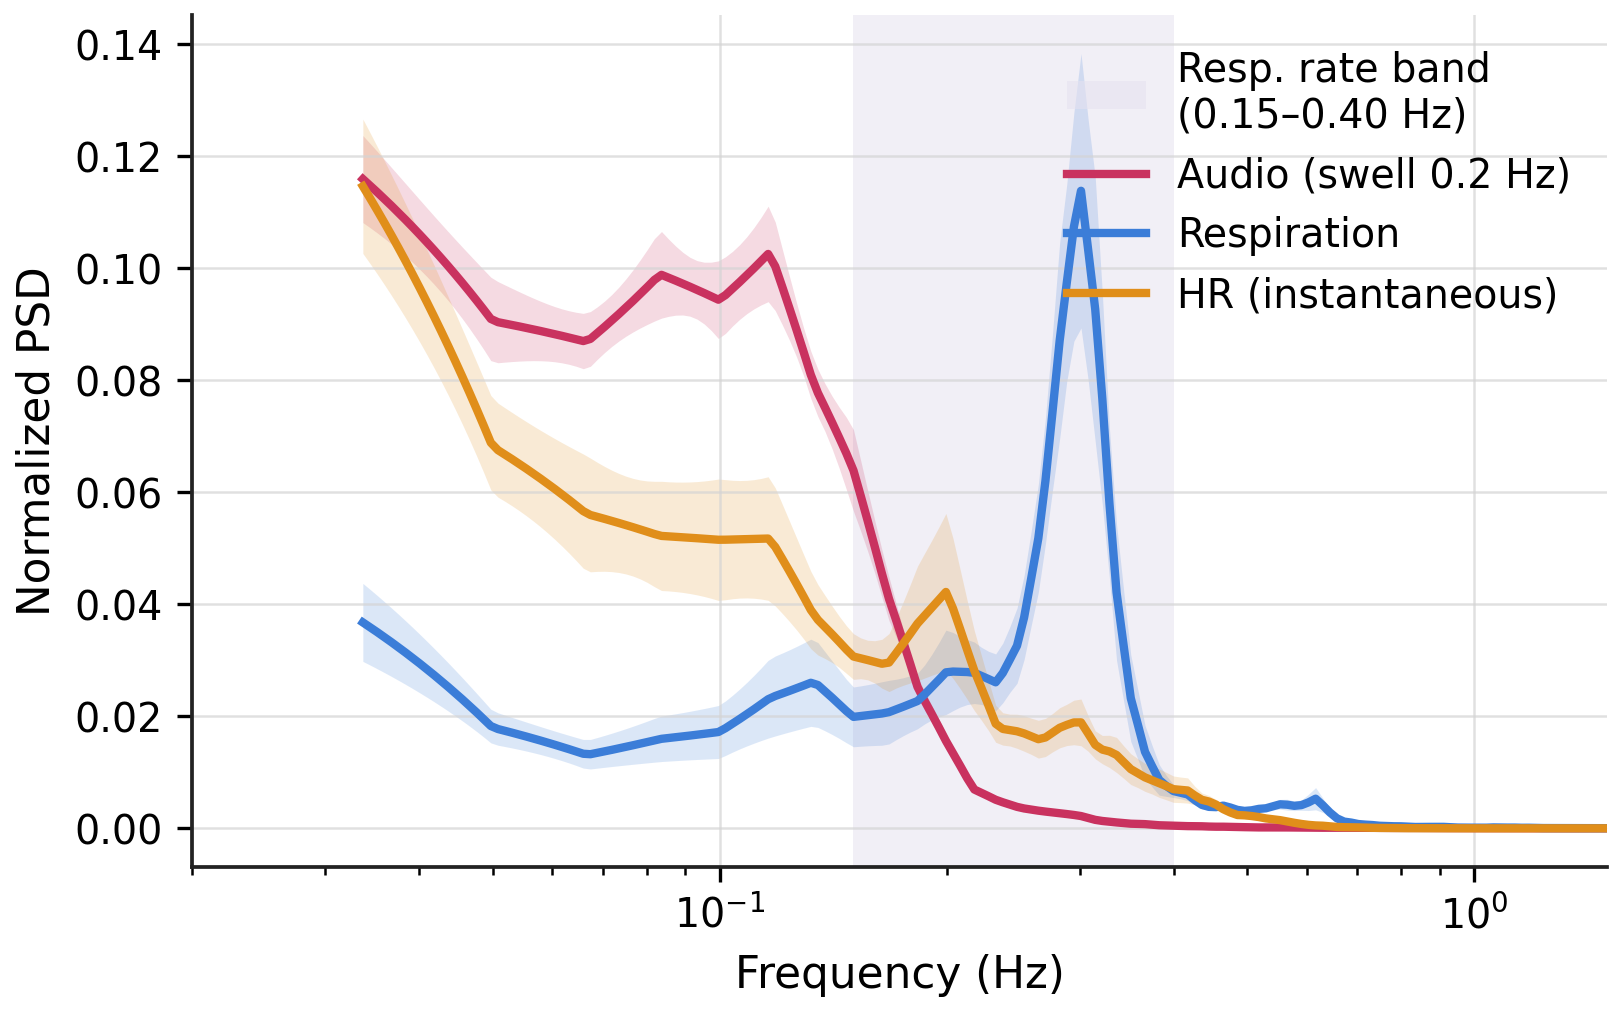
\includegraphics[width=0.85\linewidth]{A_spectrum_overlay.png}
\caption{\textbf{Audio, respiration and heart-rate spectra (group mean
$\pm$ SEM).} Welch power spectral density (PSD; 60\,s segments,
50\% overlap, Hamming window) computed per (subject, condition) and
pooled across n=5 subjects $\times$ 3 multisensory conditions
(\textsc{viz}, \textsc{aud}, \textsc{multi}; $n_{\mathrm{traces}}=15$ per
modality). PSDs were normalised to unit area in the displayed range
before averaging, then plotted on a log-frequency axis. Shaded ribbons:
SEM across the 15 traces. The lavender shaded band marks the canonical
respiratory rate range (0.15--0.40\,Hz, 9--24\,breaths/min). The audio
swell envelope (\texttt{env\_swell\_0p2}) is concentrated below 0.1\,Hz;
the respiration spectrum peaks $\sim$0.25\,Hz; instantaneous heart rate
(R-peak-derived, 4\,Hz interpolated) is broadband-slow.}
\label{fig:A}
\end{figure}

\subsection{Single-condition exemplar}

Figure~\ref{fig:alignment} illustrates the per-condition signal alignment
that drives the windowed metrics. Top: respiration and audio swell envelopes
overlaid for the first 60\,s of one \textsc{multi} block. Middle: full-signal
cross-correlation as a function of lag. Bottom: time-resolved Pearson
correlation in 30\,s sliding windows. The same three diagnostics are
generated automatically per subject and condition by the pipeline.

\begin{figure}[H]
\centering
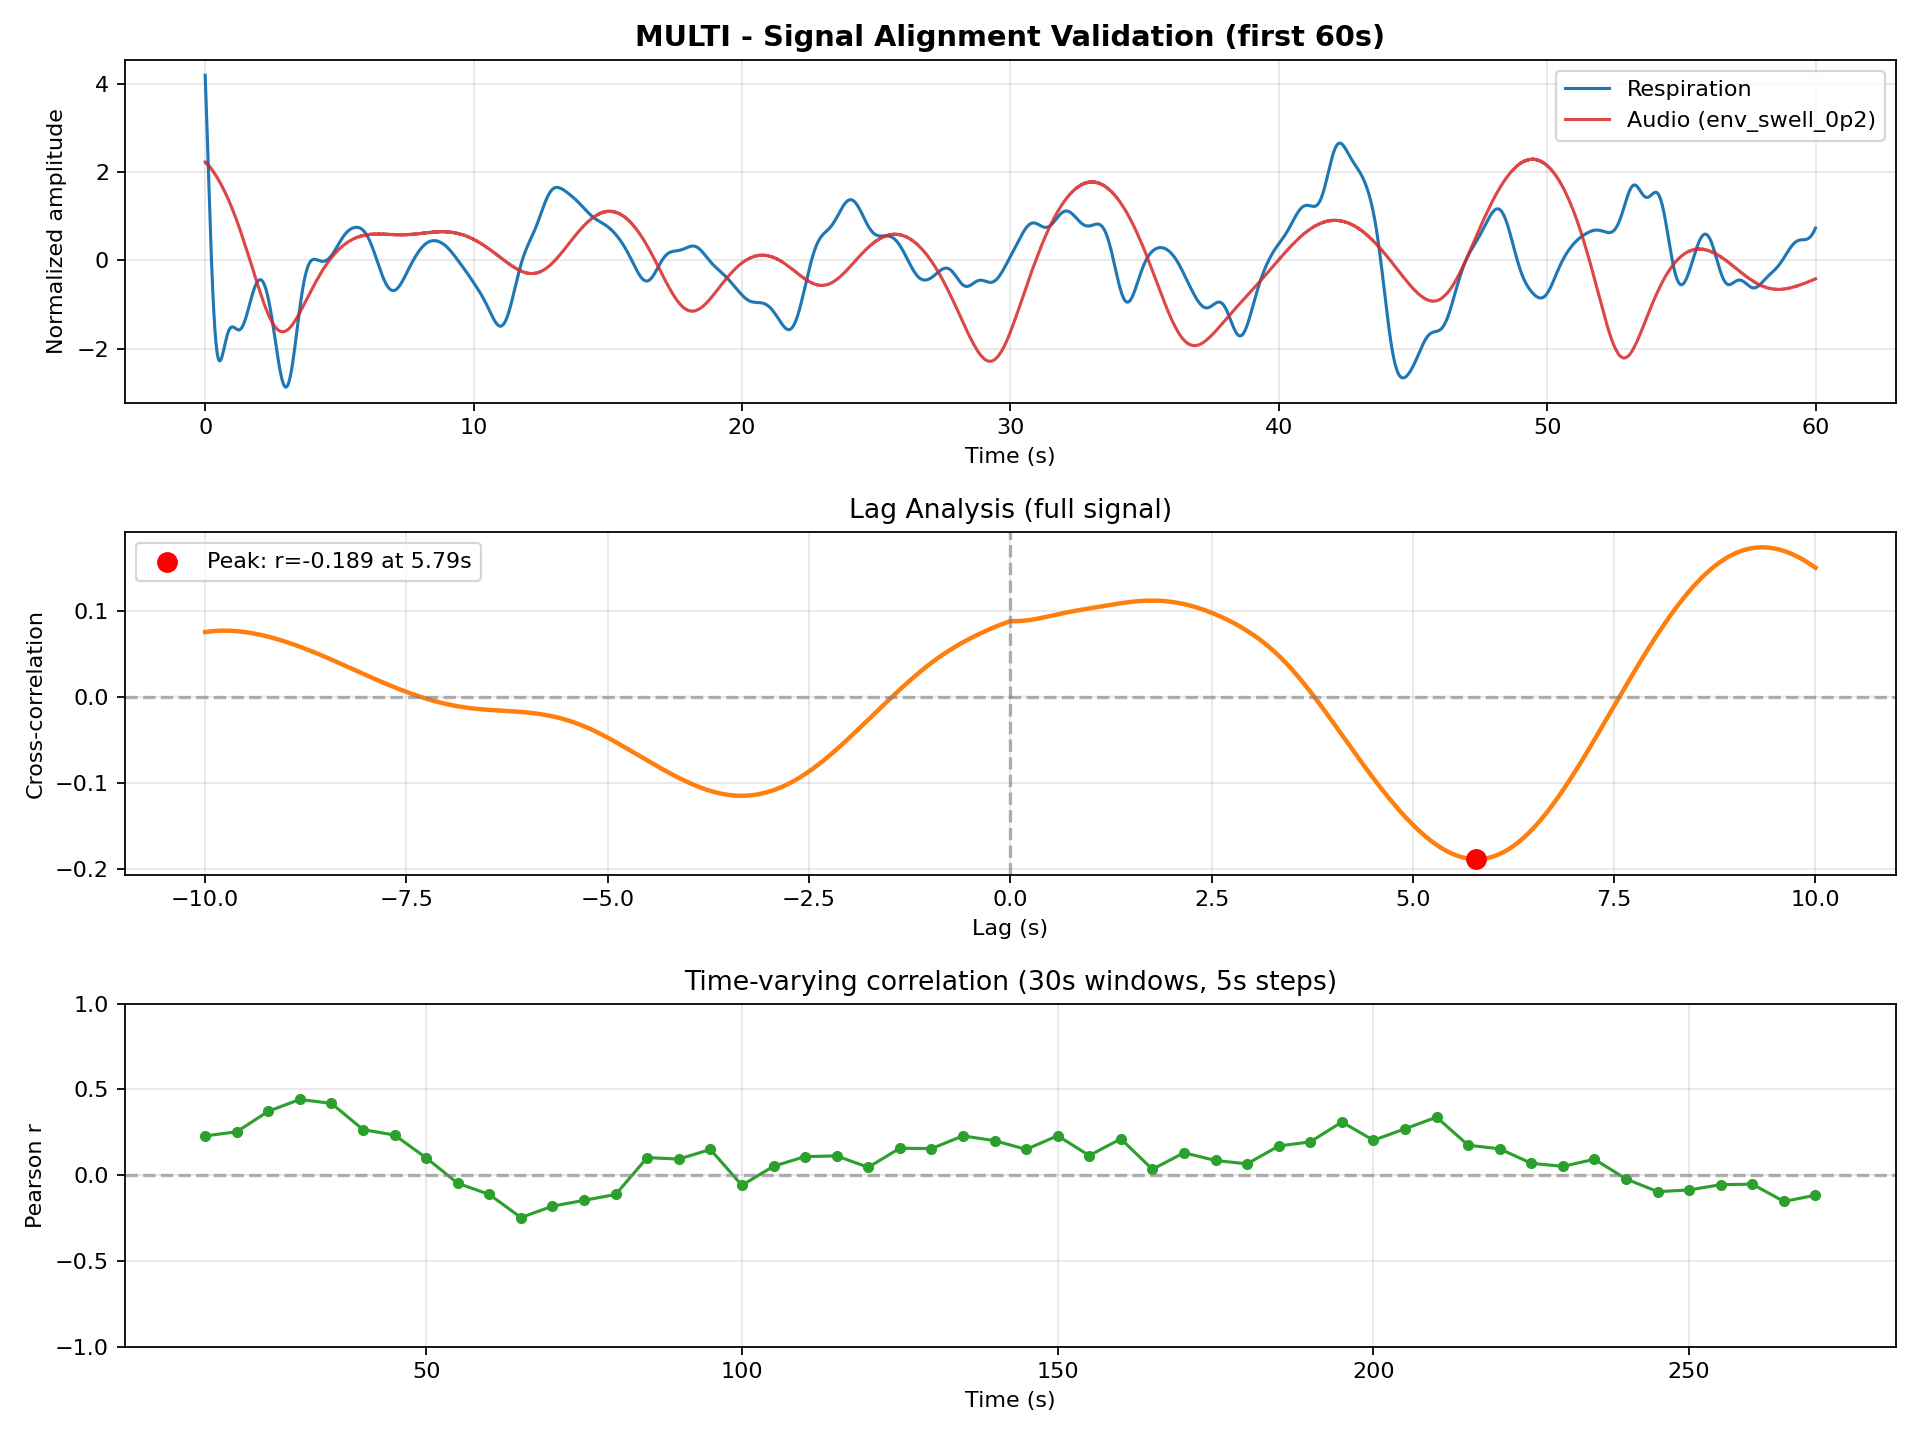
\includegraphics[width=0.85\linewidth]{alignment_figure.png}
\caption{\textbf{Per-condition alignment exemplar (sub-04, \textsc{multi}).}
\emph{Top}: cleaned respiration (blue, band-pass 0.05--1\,Hz, z-scored)
and the audio swell envelope \texttt{env\_swell\_0p2} (red, 0.2\,Hz
low-pass, log-normalised, z-scored), both at 256\,Hz, plotted over the
first 60\,s of the condition for visual inspection.
\emph{Middle}: full-segment cross-correlation as a function of lag
($\pm 10$\,s shown), normalised by signal length; the red marker shows
the maximum-amplitude peak (here $r=-0.189$ at $+5.79$\,s).
\emph{Bottom}: time-resolved Pearson $r$ in 30\,s sliding windows
(5\,s step) across the full block. The pipeline produces equivalent
diagnostics for every (subject, condition) pair as part of automated
quality-control.}
\label{fig:alignment}
\end{figure}

\subsection{Respiration and HRV: nature vs.\ rest}

Pooling \textsc{rs1}+\textsc{rs2} as ``rest'' and \textsc{viz}+\textsc{aud}+
\textsc{multi} as ``nature'' gives, per subject, two paired blocks. We
contrast the two for both respiration--audio (Figure~\ref{fig:nvr_resp}) and
HRV--audio (Figure~\ref{fig:nvr_hrv}) coupling, on the slow swell envelope
(\texttt{env\_swell\_0p2}, 0.2\,Hz low-pass).

\begin{figure}[H]
\centering
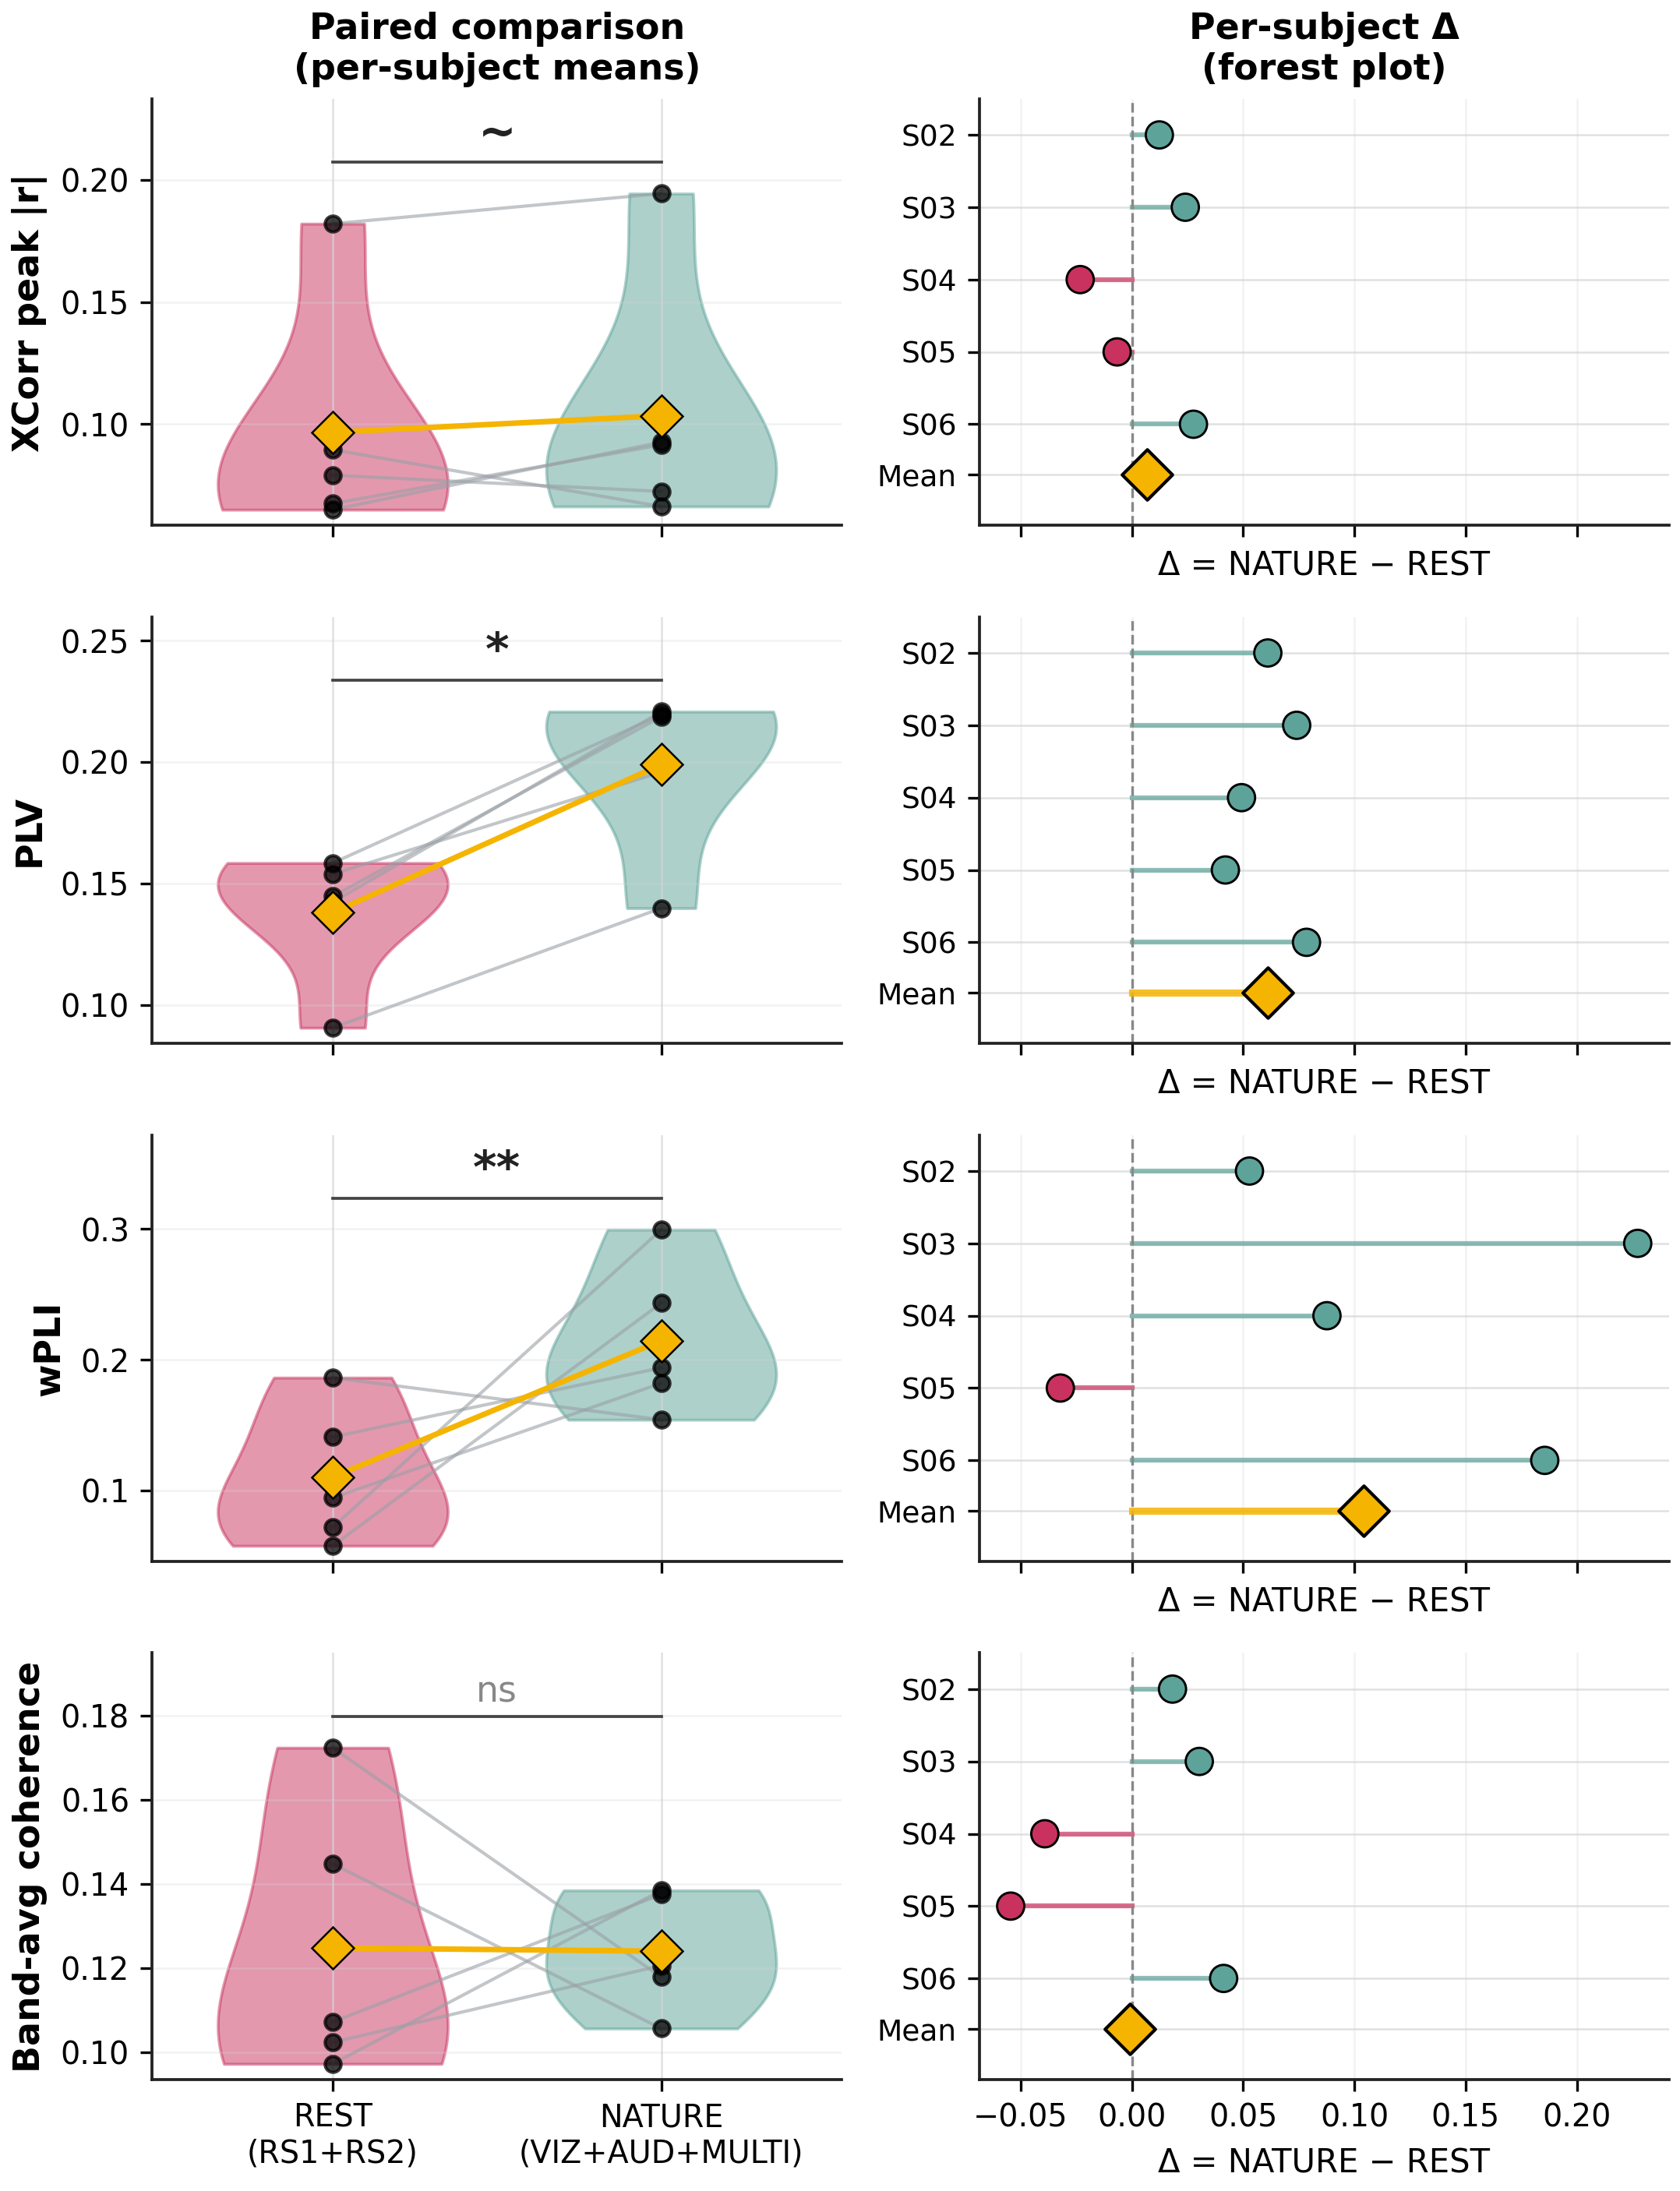
\includegraphics[width=0.95\linewidth]{Fig_nature_vs_rest_resp.png}
\caption{\textbf{Respiration--audio coupling: nature vs.\ rest
(\textsc{rs1}+\textsc{rs2} pooled vs.\ \textsc{viz}+\textsc{aud}+\textsc{multi}
pooled), n=5 subjects.} Rows: cross-correlation peak $|r|$, PLV, wPLI,
band-averaged Welch coherence (0.04--0.5\,Hz). \emph{Left}: per-subject
means as paired violins (n=5) with grey connectors and a gold mean line.
\emph{Right}: per-subject $\Delta = \mathrm{nature} - \mathrm{rest}$ as a
forest plot; green dots indicate $\Delta>0$, red $\Delta<0$; gold diamond
= group mean. Bracket stars are from a linear mixed-effects model fit on
the windowed values (metric $\sim$ block\_dummy + (1$|$subject); $\sim$440
windowed observations per metric, fitted with REML). PLV and wPLI rise
consistently under nature (LMM $p=0.027$ and $p=0.0067$ respectively);
cross-correlation shows a trend ($p=0.066$, $\sim$); coherence is
unchanged. Significance code: \texttt{*** $p\!<\!.001$,
** $p\!<\!.01$, * $p\!<\!.05$, $\sim$ $p\!<\!.10$, ns} otherwise.}
\label{fig:nvr_resp}
\end{figure}

\begin{figure}[H]
\centering

\includegraphics[width=0.95\linewidth]{Fig_nature_vs_rest_hrv_meannn.png}
\caption{\textbf{HRV (mean NN interval)--audio coupling: nature vs.\ rest,
n=5 subjects.} Same layout and statistical apparatus as
Figure~\ref{fig:nvr_resp}. HRV time series: per-window mean RR interval
from R-peak detection on cleaned ECG (NeuroKit2), interpolated to 4\,Hz.
Audio: \texttt{env\_swell\_0p2} envelope resampled to the HRV grid by
linear interpolation. With the 0.2\,Hz swell envelope, mean RR-interval
coupling does not differ between rest and nature on any metric (LMM
$p \geq 0.15$ in all four panels). The multi-envelope sweep
(Figure~\ref{fig:F_hrv}) locates HRV's strongest coupling at the
very-slow 0.1\,Hz swell, where it \emph{decouples} during nature
(supplementary recompute on \texttt{env\_swell\_0p1}: PLV $p=0.064$,
wPLI $p=0.018$, both \emph{negative} $\Delta$).}
\label{fig:nvr_hrv}
\end{figure}

\subsection{Three-condition contrast: PLV / wPLI / coherence}

Within the multisensory comparison itself (Figure~\ref{fig:fig5_resp},
respiration; Figure~\ref{fig:fig5_hrv}, HRV mean NN), the audio-only
condition shows the strongest respiration--audio coupling on phase metrics,
peaking $\sim$2$\times$ the value seen during \textsc{viz} or \textsc{multi}.
The omnibus Friedman test does not reach $p\!<\!0.05$ at n=5
($p_{\mathrm{wPLI}}=0.165$), but pairwise Wilcoxon comparisons show
\textsc{viz}--\textsc{aud} as the dominant trend. HRV-mean-NN coupling shows
a significant Friedman effect on wPLI ($p=0.022$, $*$).

\begin{figure}[H]
\centering
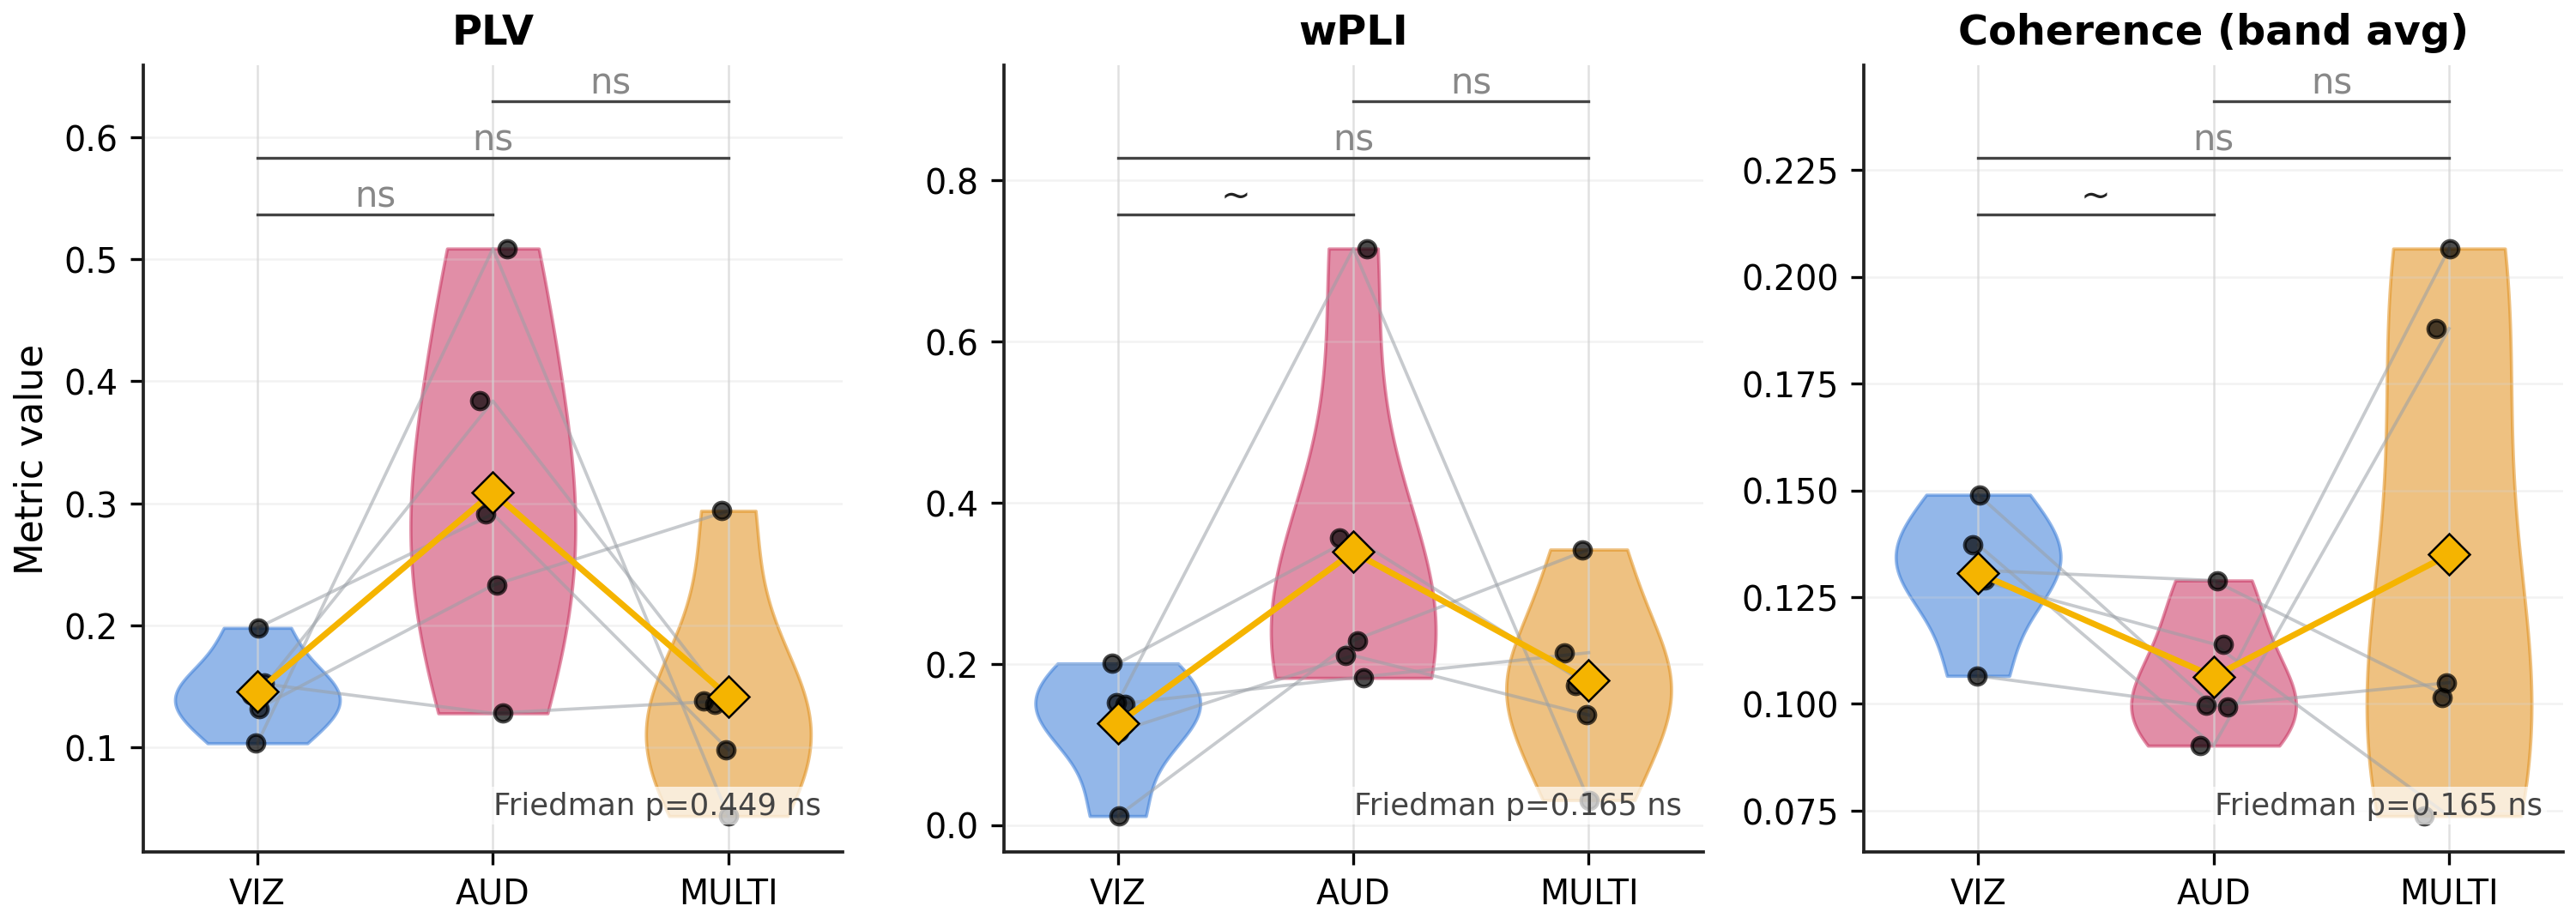
\includegraphics[width=0.95\linewidth]{Fig5_resp_audio_metrics_grid.png}
\caption{\textbf{Respiration--audio coupling across the three multisensory
conditions, n=5 subjects.} Per-subject whole-block scalars for PLV, wPLI
and band-averaged coherence (0.04--0.5\,Hz Welch). Each panel: violins
of the n=5 subject means per condition; grey lines connect paired
within-subject values; gold diamond + line shows the group mean.
Statistics: Friedman test (omnibus, n=5, df=2; reported inline per panel),
followed by all three pairwise Wilcoxon signed-rank post-hoc tests (paired,
two-sided) shown as brackets above the violins. Significance code:
\texttt{*** $p\!<\!.001$, ** $p\!<\!.01$, * $p\!<\!.05$,
$\sim$ $p\!<\!.10$, ns} otherwise. With n=5 the Friedman omnibus is
under-powered and does not reach $p\!<\!0.05$ on PLV or wPLI ($p=0.165$
each), but pairwise comparisons identify \textsc{viz} vs.\ \textsc{aud}
as the dominant contrast on wPLI ($\sim$).}
\label{fig:fig5_resp}
\end{figure}

\begin{figure}[H]
\centering

\includegraphics[width=0.95\linewidth]{Fig5_HRV_audio_metrics_grid.png}
\caption{\textbf{HRV (mean NN)--audio coupling across the three multisensory
conditions, n=5 subjects.} Same layout and statistical apparatus as
Figure~\ref{fig:fig5_resp} (Friedman omnibus + three pairwise Wilcoxon
post-hoc; same significance code). HRV mean NN interval was extracted in
30\,s rolling windows (90\% overlap) via NeuroKit2 and interpolated to
4\,Hz. wPLI shows a significant Friedman effect ($\chi^2(2)$, $p=0.022$,
$*$), with the \textsc{viz}--\textsc{aud} pair carrying the trend
($p=0.06$, $\sim$). PLV and band-averaged coherence are not significant
across conditions.}
\label{fig:fig5_hrv}
\end{figure}

\subsection{Phase clustering across subjects (hierarchical Rayleigh)}

For each (subject, condition) we extract $\sim$20 windowed preferred phases
(from the windowed PLV) and run a within-subject Rayleigh test: subjects
classified as ``locked'' if their windowed phases concentrate
($p\!<\!0.05$). Group-level Rayleigh on the per-subject mean phases tests
whether subjects collectively converge on a similar phase
(Figure~\ref{fig:E}). Both within-subject and group-level locking are
maximal under \textsc{aud} (4/5 subjects locked, group $R=0.73$,
Rayleigh $p=0.060$, trend), and lowest under \textsc{multi}
(group $R=0.22$, $p=0.808$). Visual stimulation alone shows an intermediate
profile.

\begin{figure}[H]
\centering
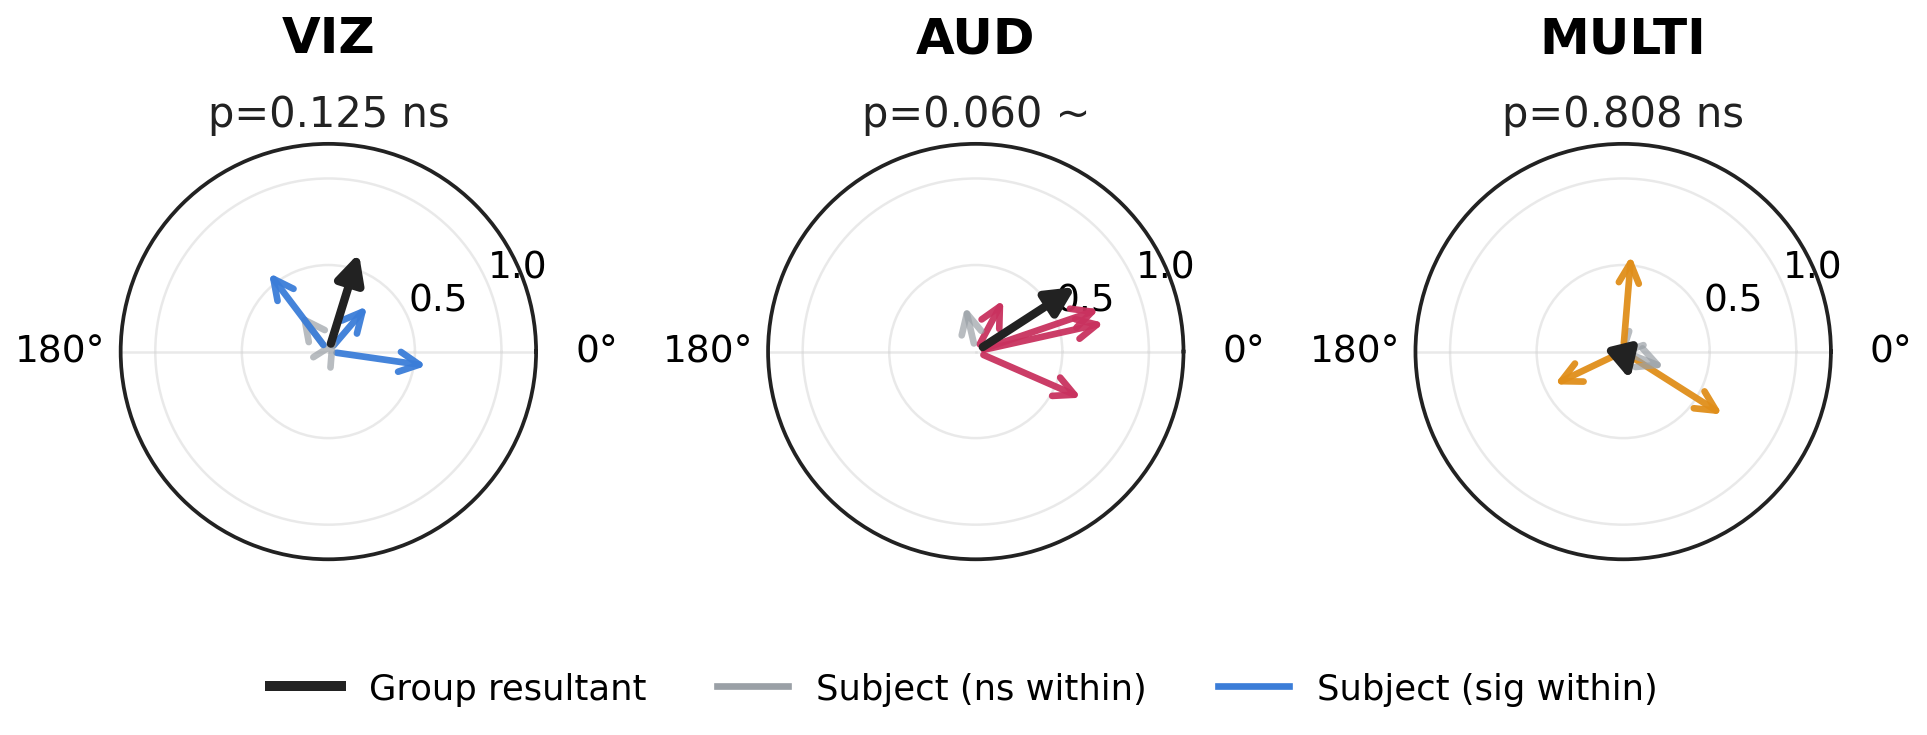
\includegraphics[width=0.95\linewidth]{E_phase_polar.png}
\caption{\textbf{Hierarchical phase consistency: respiration vs.\ audio
swell envelope (\texttt{env\_swell\_0p2}), n=5 subjects.} Each subject's
PLV pipeline produces $\sim$20 windowed preferred phases per condition
(120\,s window, 10\,s step at 256\,Hz). \emph{Within-subject layer}: a
Rayleigh test on each subject's $\sim$20 phases yields a per-subject
resultant length $R$ and a $p$-value; arrows in colour are
\emph{within}-subject significant ($p\!<\!0.05$), grey otherwise. Each
arrow is drawn at the subject's circular-mean phase with length $R$.
\emph{Group-level layer}: a second Rayleigh on the n=5 subject-mean
phases tests whether the group converges on a common phase; the black
arrow shows the group mean resultant, panel header reports the group $R$
and $p$. Audio-only gives the tightest clustering (4/5 within-subject
significant; group $R=0.73$, $p=0.060$, $\sim$); audio--visual gives the
loosest ($R=0.22$, $p=0.808$, ns). Significance code as in
Figure~\ref{fig:nvr_resp}.}
\label{fig:E}
\end{figure}

\subsection{Multi-envelope coupling fingerprint}

Sweeping all four coupling metrics against all 12 audio-band envelopes
(Figures~\ref{fig:F_resp} and \ref{fig:F_hrv}) gives a per-modality
fingerprint of where in the audio's frequency hierarchy the coupling lives.
For respiration, phase-based metrics (PLV, wPLI) lock most strongly to the
slow swell envelopes and to the band that overlaps the breathing rate
(0.15--0.40\,Hz HRV-HF band). For HRV mean NN, mutual information dominates
on the slow swells (values $\geq 0.7$) but is essentially zero on the EEG
bands --- biologically expected, because the heart-rate signal cannot share
information with audio amplitude modulations at, e.g., 8--13\,Hz that have
no counterpart in cardiac dynamics.

\begin{figure}[H]
\centering
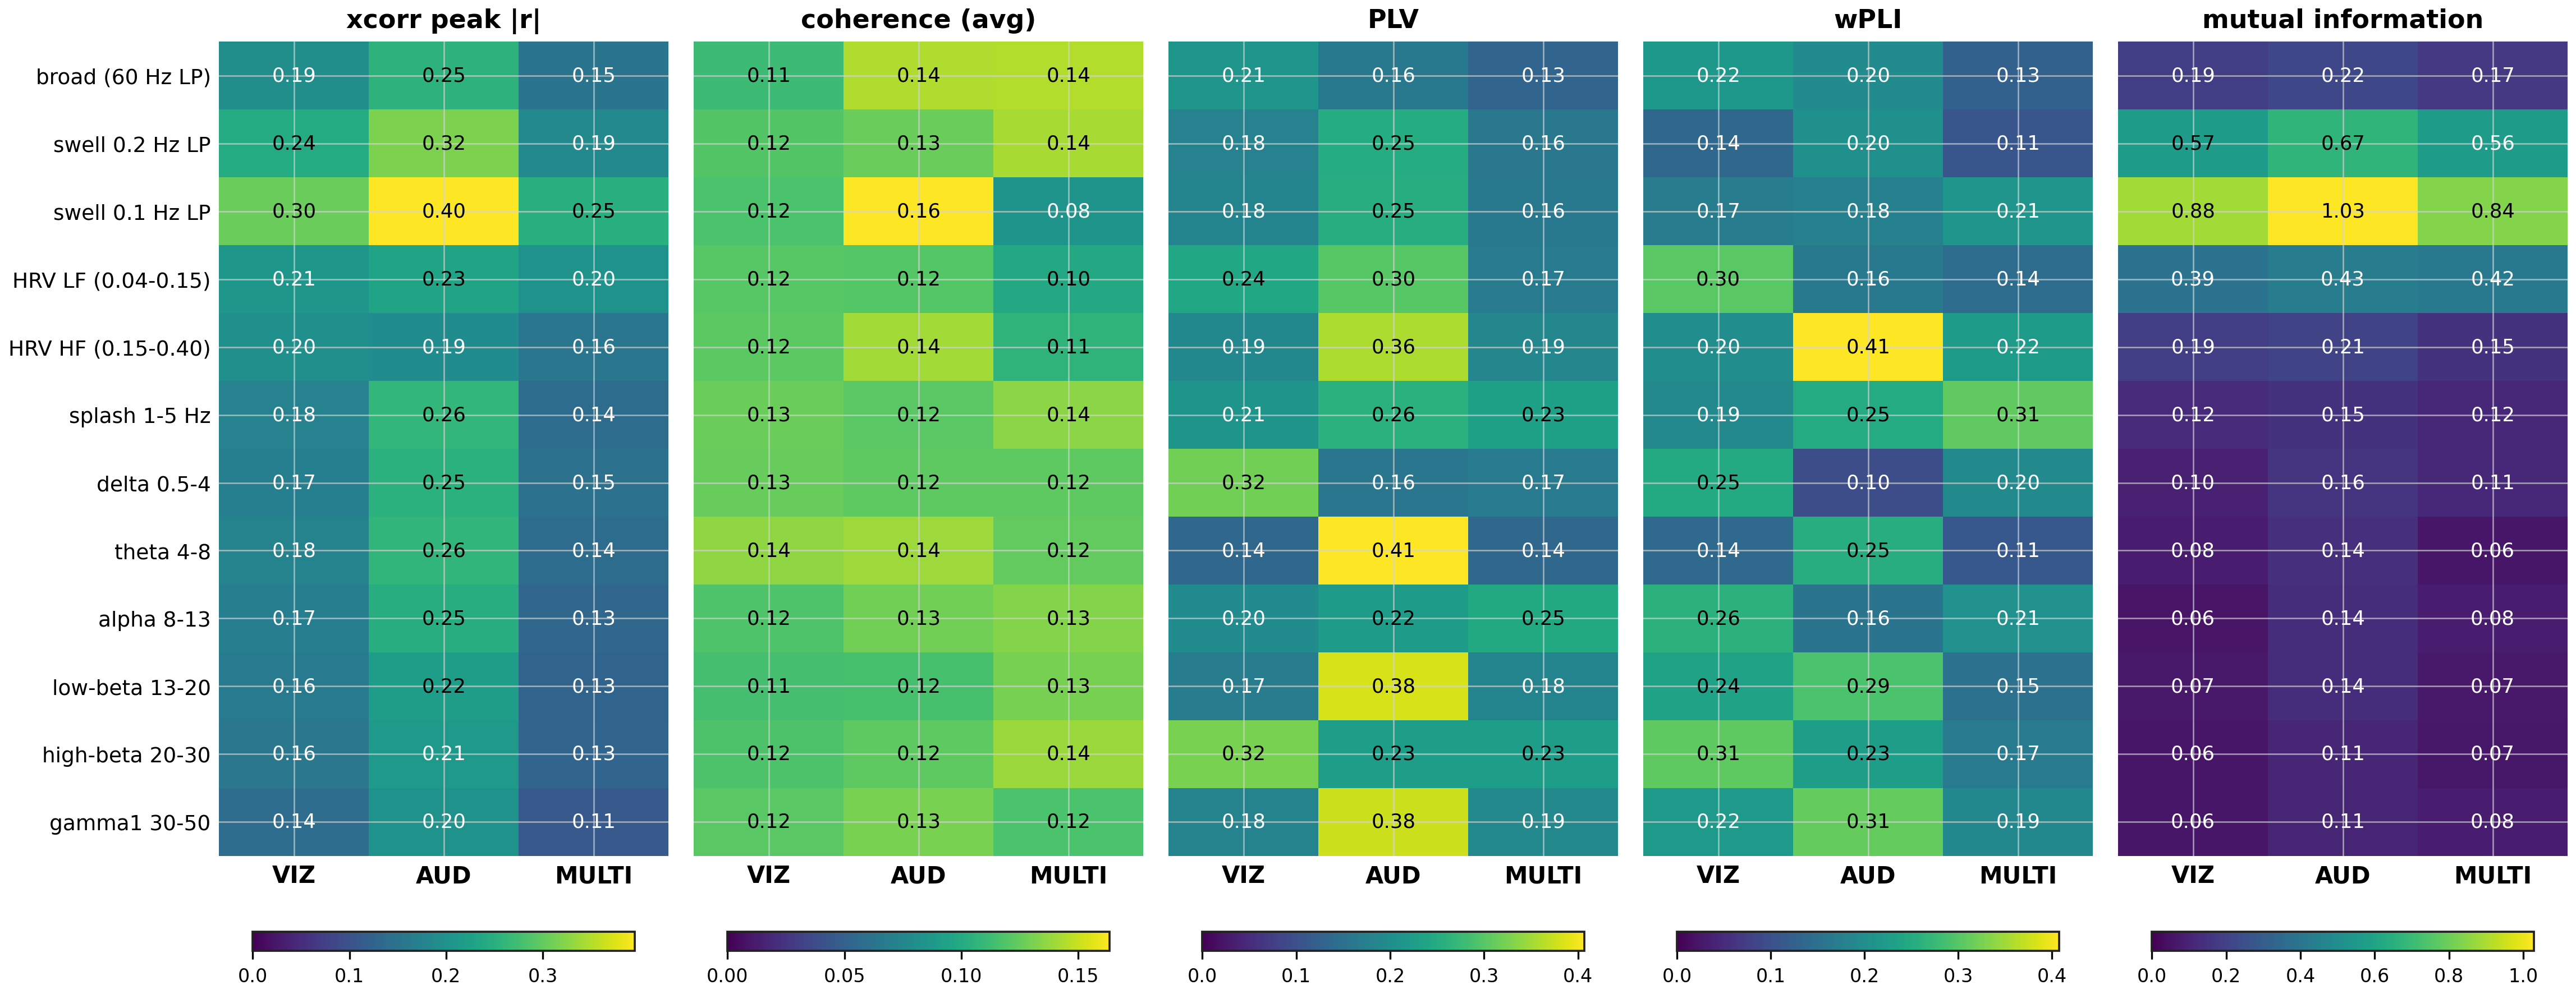
\includegraphics[width=0.96\linewidth]{F_HRV_multi_envelope_heatmap_HRV_MeanNN.png}
\caption{\textbf{HRV (mean NN)--audio coupling fingerprint, n=5 subjects.}
Group-mean coupling per (audio-band envelope $\times$ coupling method
$\times$ multisensory condition). Rows = the 12 band-organised audio
envelope columns (broadband, two slow swells, two HRV-band envelopes,
splash band, six EEG bands); columns within each metric panel = the three
conditions (\textsc{viz}, \textsc{aud}, \textsc{multi}); panels = the five
coupling methods (xcorr peak $|r|$, band-averaged coherence, PLV, wPLI,
mutual information). Each metric panel has its own colour scale (printed
under the colourbar) so within-metric variation across bands is visible.
Mutual information dominates on the slow swells (values 0.7--1.0,
upward-biased by autocorrelation but consistent across conditions).
Phase metrics (PLV, wPLI) peak around the HRV-LF/HF range
(0.04--0.40\,Hz), supporting the interpretation that HRV coupling is
strongest in the autonomic-rhythm band.}
\label{fig:F_hrv}
\end{figure}

\begin{figure}[H]
\centering
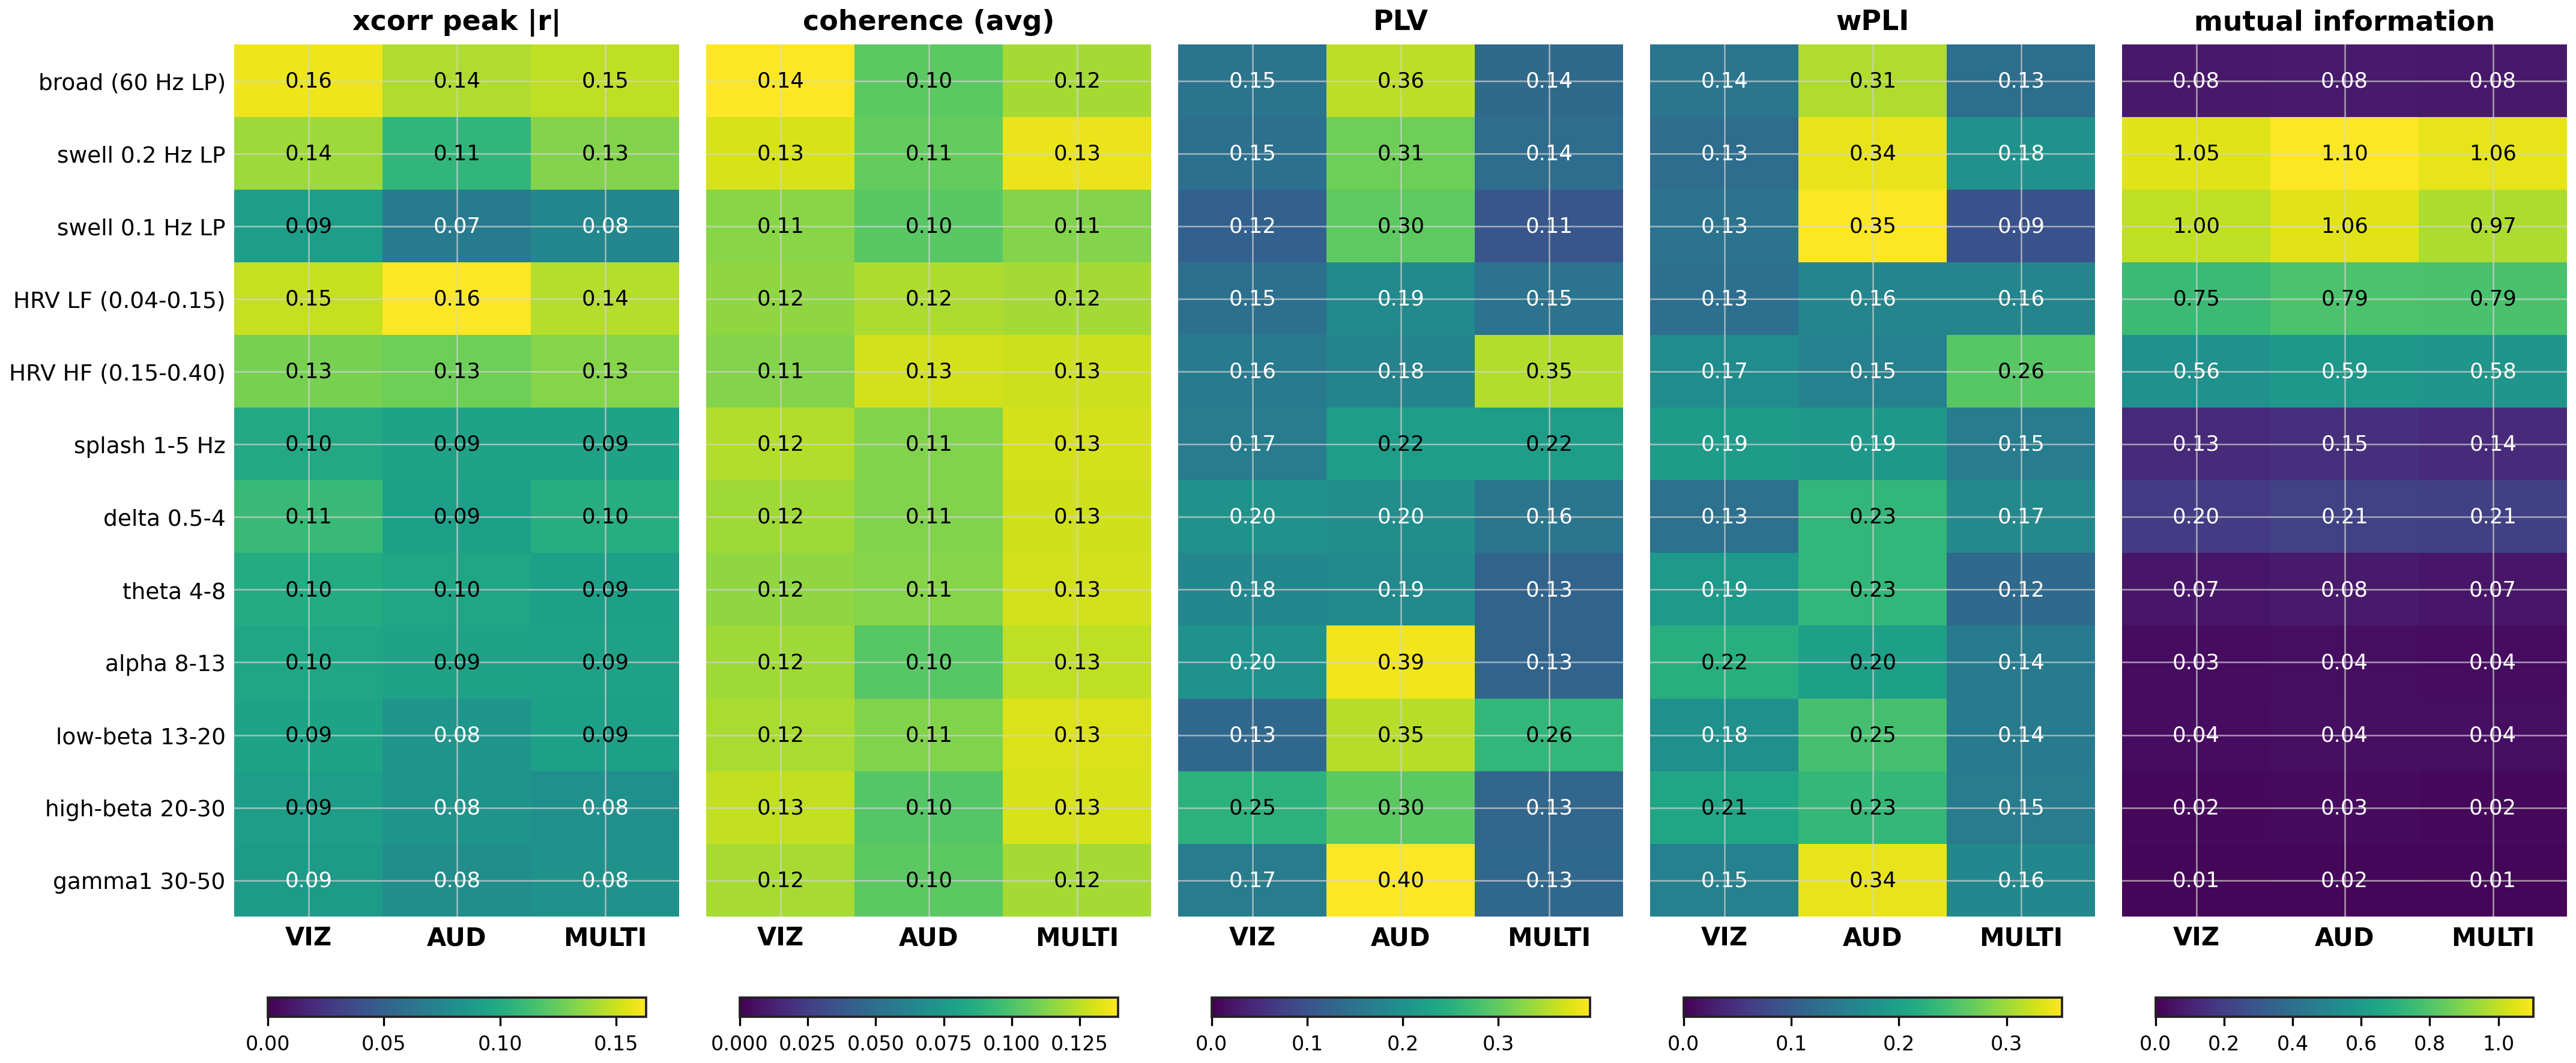
\includegraphics[width=0.96\linewidth]{F_multi_envelope_heatmap.png}
\caption{\textbf{Respiration--audio coupling fingerprint, n=5 subjects.}
Same layout as Figure~\ref{fig:F_hrv}, with cleaned respiration
(0.05--1\,Hz band-pass + z-score) as the source signal at 256\,Hz. PLV and
wPLI are highest on the slow-swell envelopes (\texttt{env\_swell\_0p1} and
\texttt{env\_swell\_0p2}) and on the HRV-HF band envelope
(0.15--0.40\,Hz) that overlaps the breathing rate; cross-correlation and
band-averaged coherence are flat across bands. MI is highest on the slow
swells (autocorrelation-biased; valid for relative comparison).}
\label{fig:F_resp}
\end{figure}

\subsection{Time-resolved coupling within condition}

Aggregating the windowed PLV, wPLI and band-averaged coherence over
normalised time within each condition (Figure~\ref{fig:C_plv},
\ref{fig:C_wpli}, \ref{fig:C_coh}) shows that respiration--audio phase
coupling \emph{builds up} during \textsc{aud} listening (per-subject linear
slope, Wilcoxon vs.\ 0): coherence $p\!=\!0.063$ (trend) and wPLI/PLV with
positive trend; the same trajectory is largely flat for \textsc{viz} and
\textsc{multi}.

\begin{figure}[H]
\centering
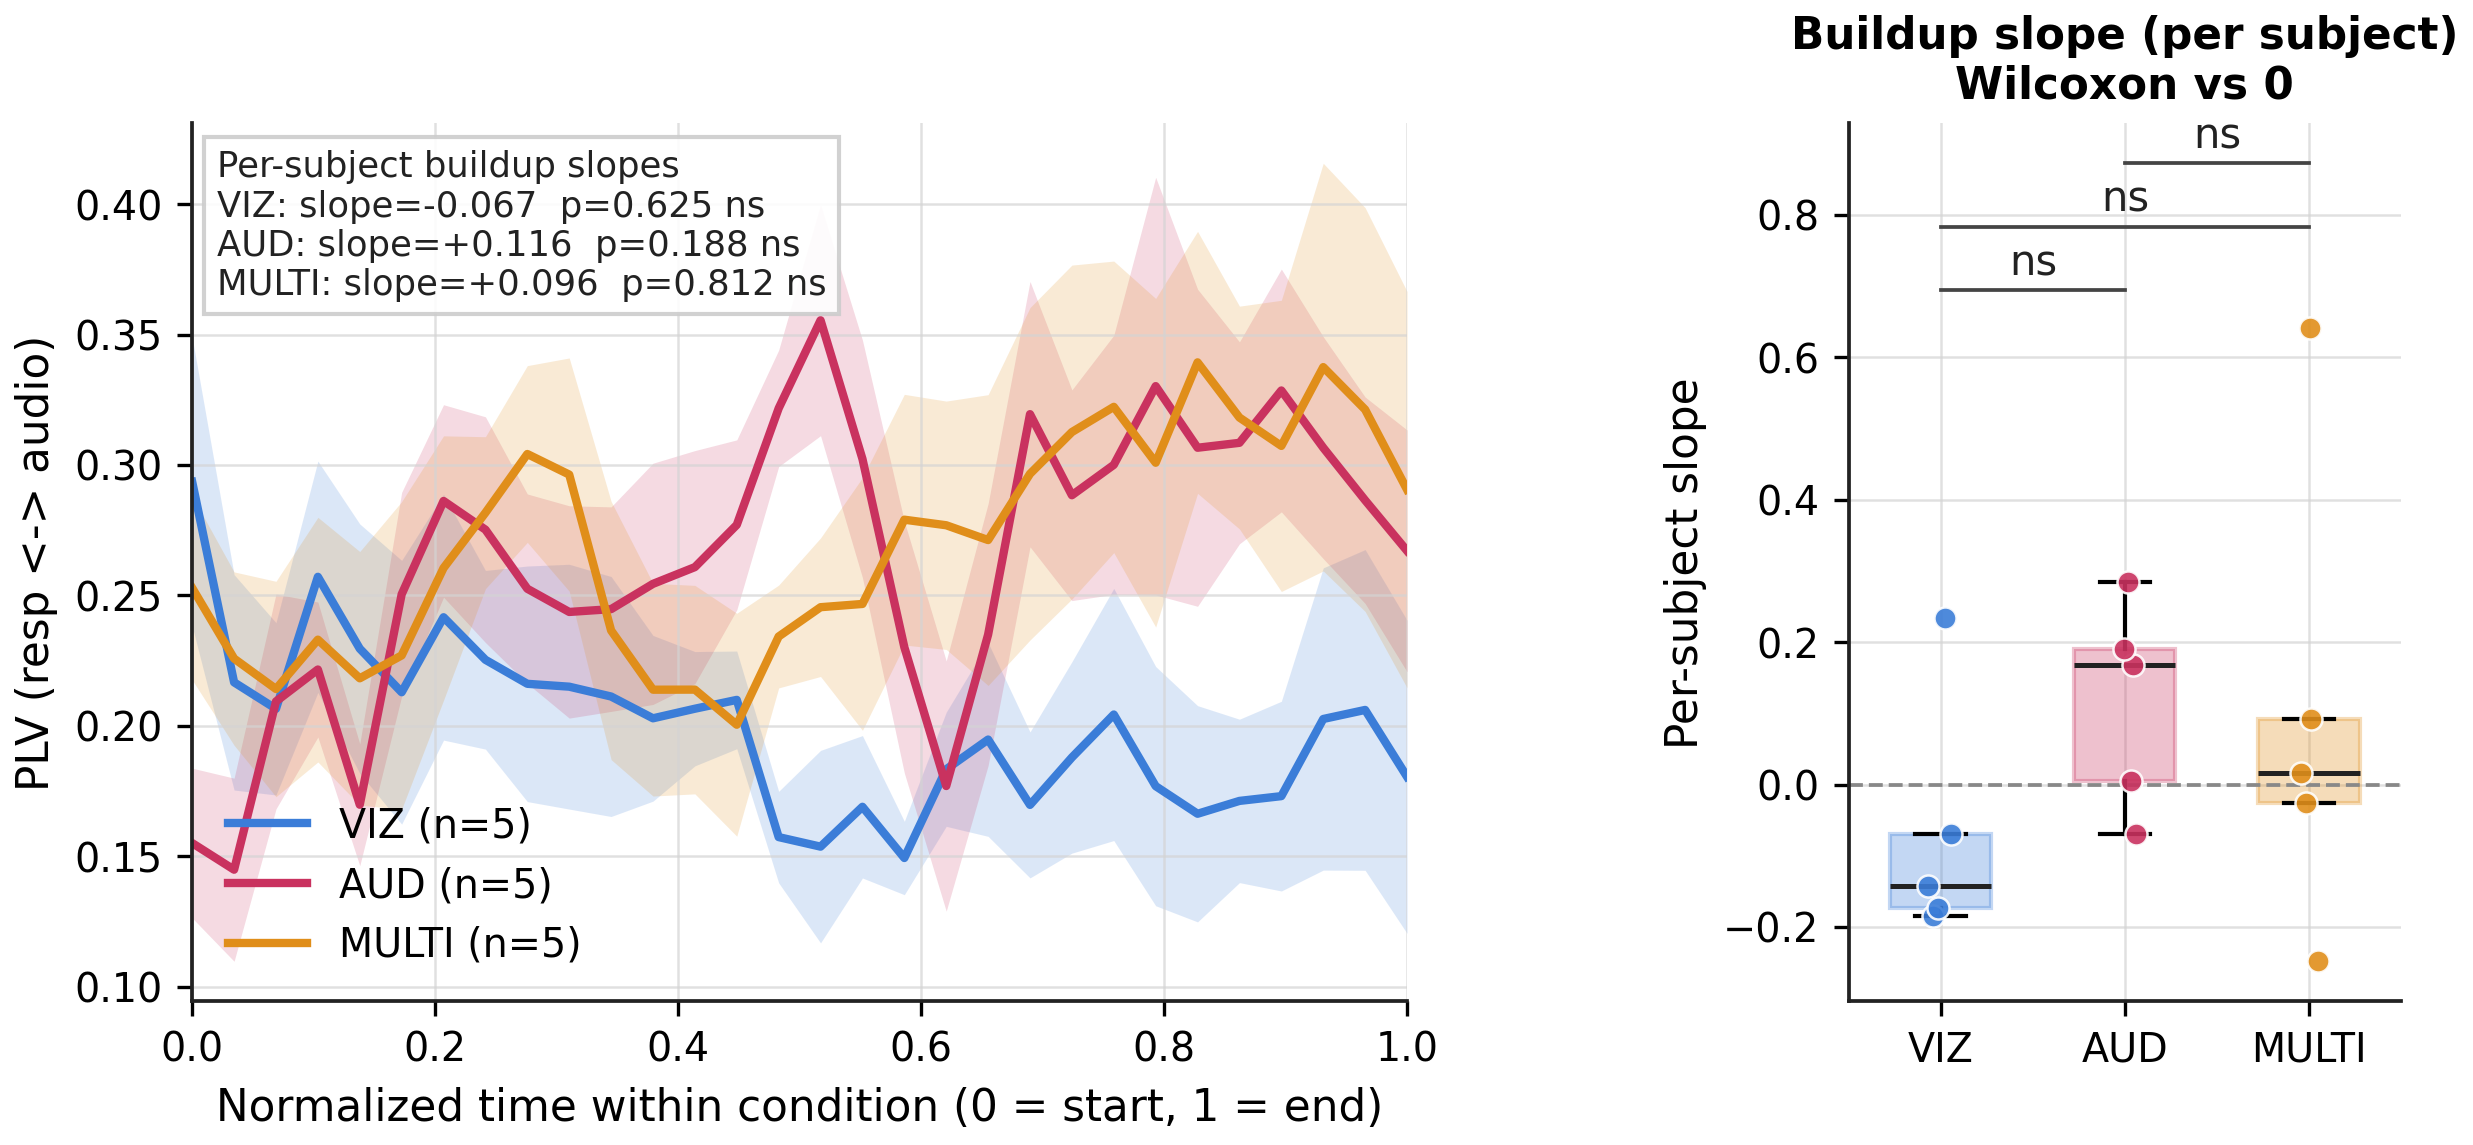
\includegraphics[width=0.92\linewidth]{C_time_resolved_resp_audio_plv.png}
\caption{\textbf{Time-resolved PLV (respiration vs.\ audio swell), n=5
subjects.} \emph{Left}: per-condition group mean $\pm$ SEM PLV trajectory
across normalised time within the condition (each subject's $\sim$20
windowed PLV values resampled to 30 evenly-spaced bins covering [0, 1]
from condition start to end). \emph{Right}: per-subject linear-trend slope
of the PLV time series within each condition (one slope per subject from
\texttt{scipy.stats.linregress} on the normalised time axis); boxplot +
dots show the n=5 distribution. The header reports the one-sample
Wilcoxon test of slope $\neq 0$ per condition. Pairwise brackets between
conditions are paired Wilcoxon tests on the slopes. Audio-only shows the
strongest positive build-up (mean slope $+0.12$).}
\label{fig:C_plv}
\end{figure}

\begin{figure}[H]
\centering
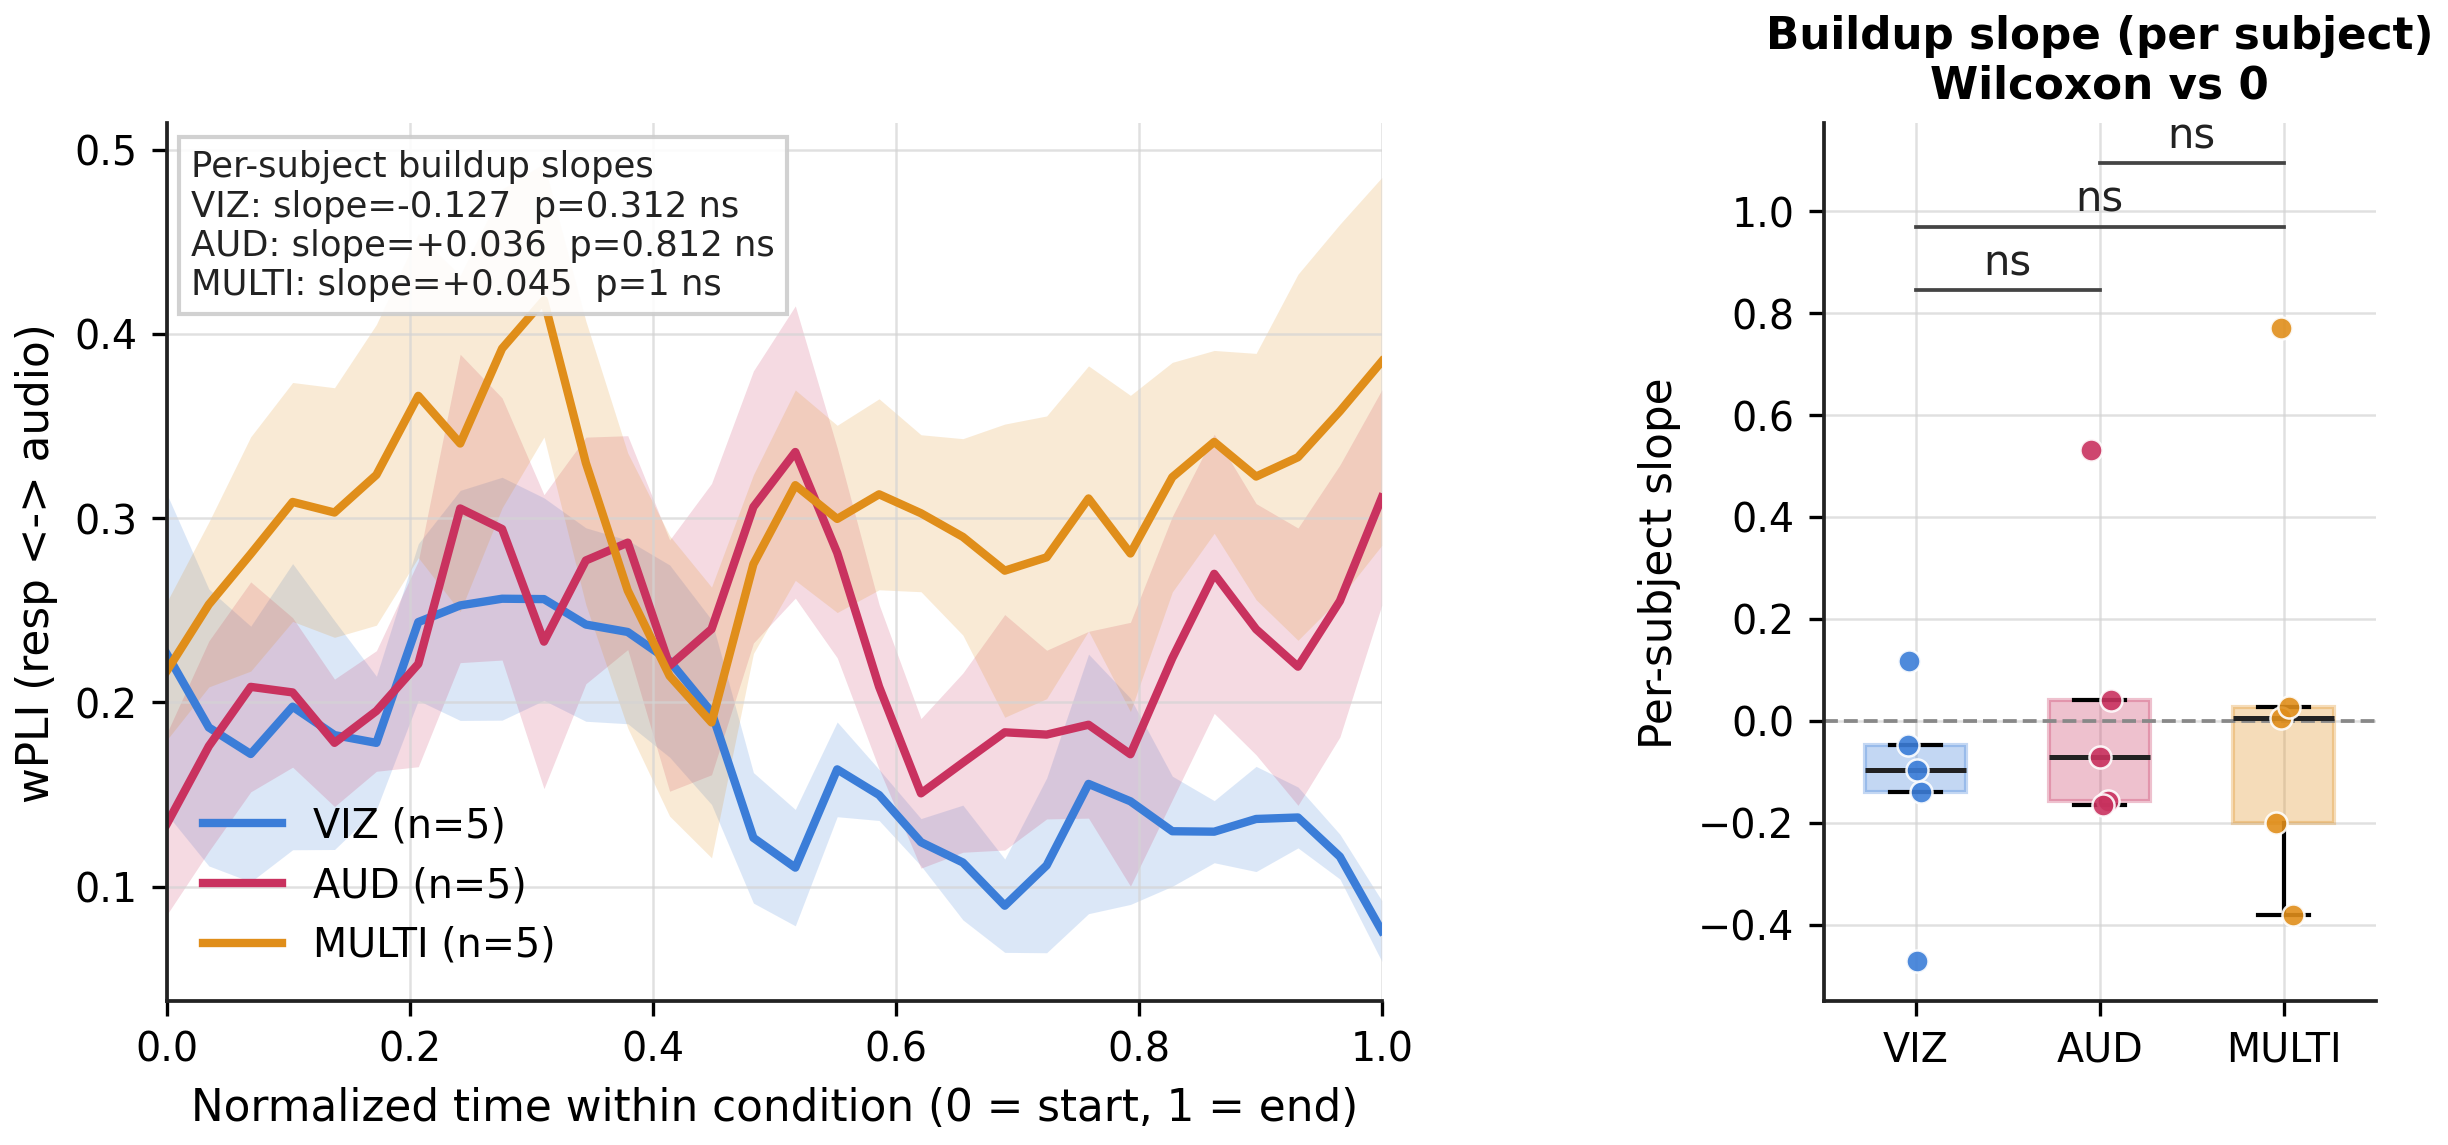
\includegraphics[width=0.92\linewidth]{C_time_resolved_resp_audio_wpli.png}
\caption{\textbf{Time-resolved wPLI (respiration vs.\ audio swell), n=5
subjects.} Same layout and statistical apparatus as
Figure~\ref{fig:C_plv}. wPLI shows a similar audio-only build-up
trajectory but with greater between-subject variability than PLV.}
\label{fig:C_wpli}
\end{figure}

\begin{figure}[H]
\centering
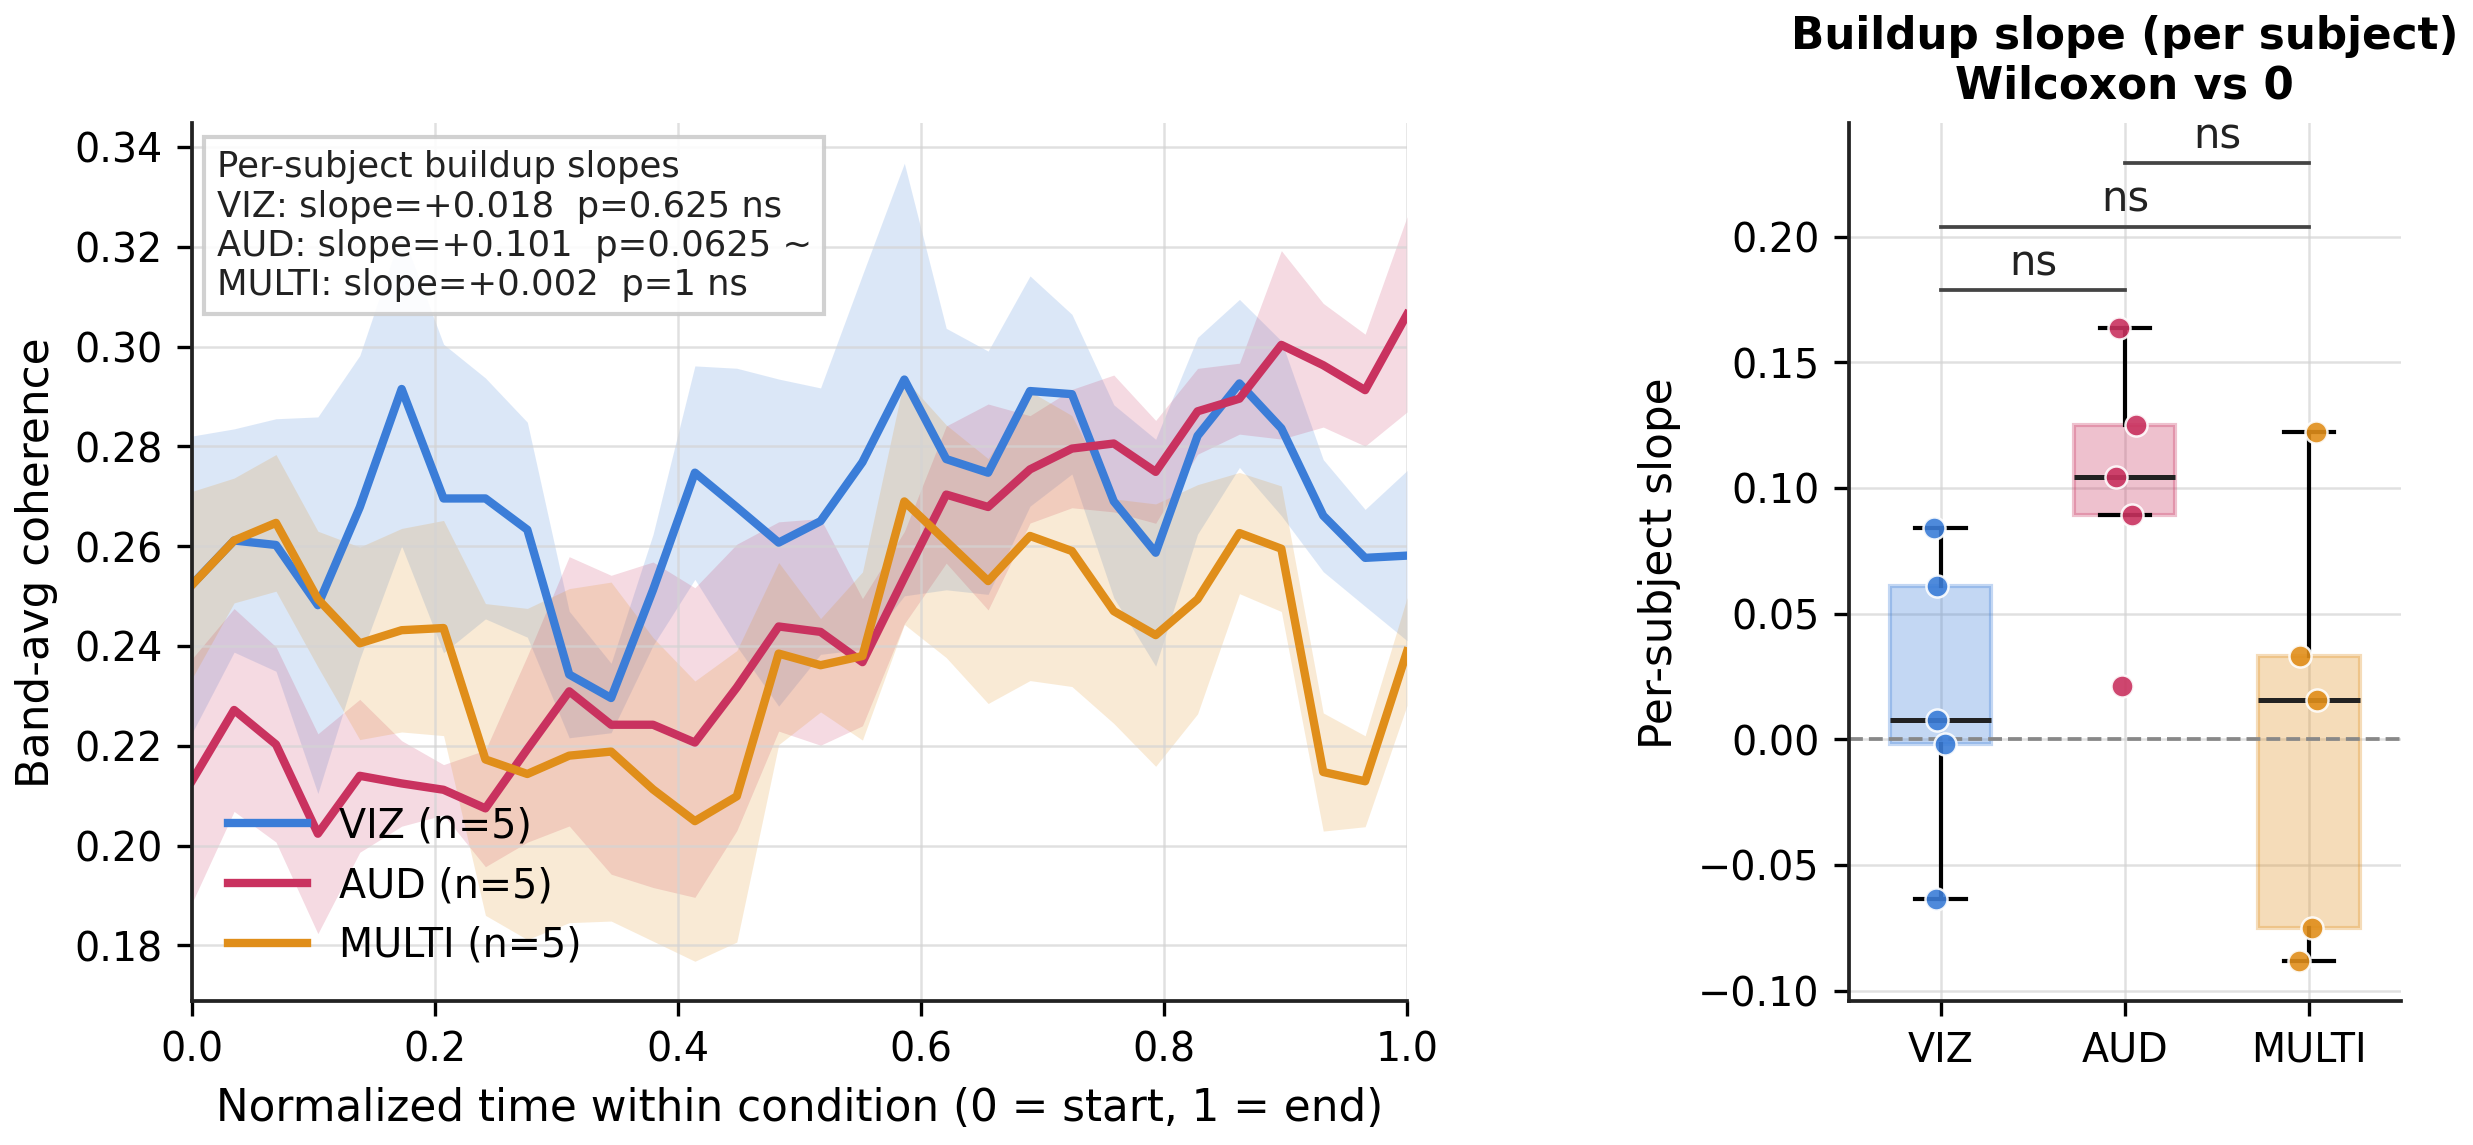
\includegraphics[width=0.92\linewidth]{C_time_resolved_resp_audio_coh.png}
\caption{\textbf{Time-resolved band-averaged coherence (respiration vs.\
audio swell), n=5 subjects.} Same layout and statistical apparatus as
Figure~\ref{fig:C_plv}. Coherence is averaged over 0.04--0.5\,Hz per
sliding window. Audio-only listening shows a positive build-up slope
(per-subject Wilcoxon vs.\ zero $p=0.063$, $\sim$).}
\label{fig:C_coh}
\end{figure}

\subsection{EEG--audio band-matched correlation}

For each EEG band we band-pass-filter the audio envelope and the EEG to
the same band, then compute per-channel Pearson correlations. Linear
mixed-effects per channel + FDR across the 32 channels per band reveal
band-specific differences between conditions
(Figure~\ref{fig:Fig4_VA}, \ref{fig:Fig4_VM}, \ref{fig:Fig4_AM}). The
strongest contrasts are in delta (\textsc{viz} vs.\ \textsc{aud}: 30/32
channels FDR $<\!.05$, $*$), alpha (\textsc{viz} vs.\ \textsc{aud}:
32/32, $***$), and high-beta (11/32, $*$). Pairs of conditions involving
\textsc{multi} also engage theta (23/32 channels for \textsc{viz} vs.\
\textsc{multi}).

\begin{figure}[H]
\centering
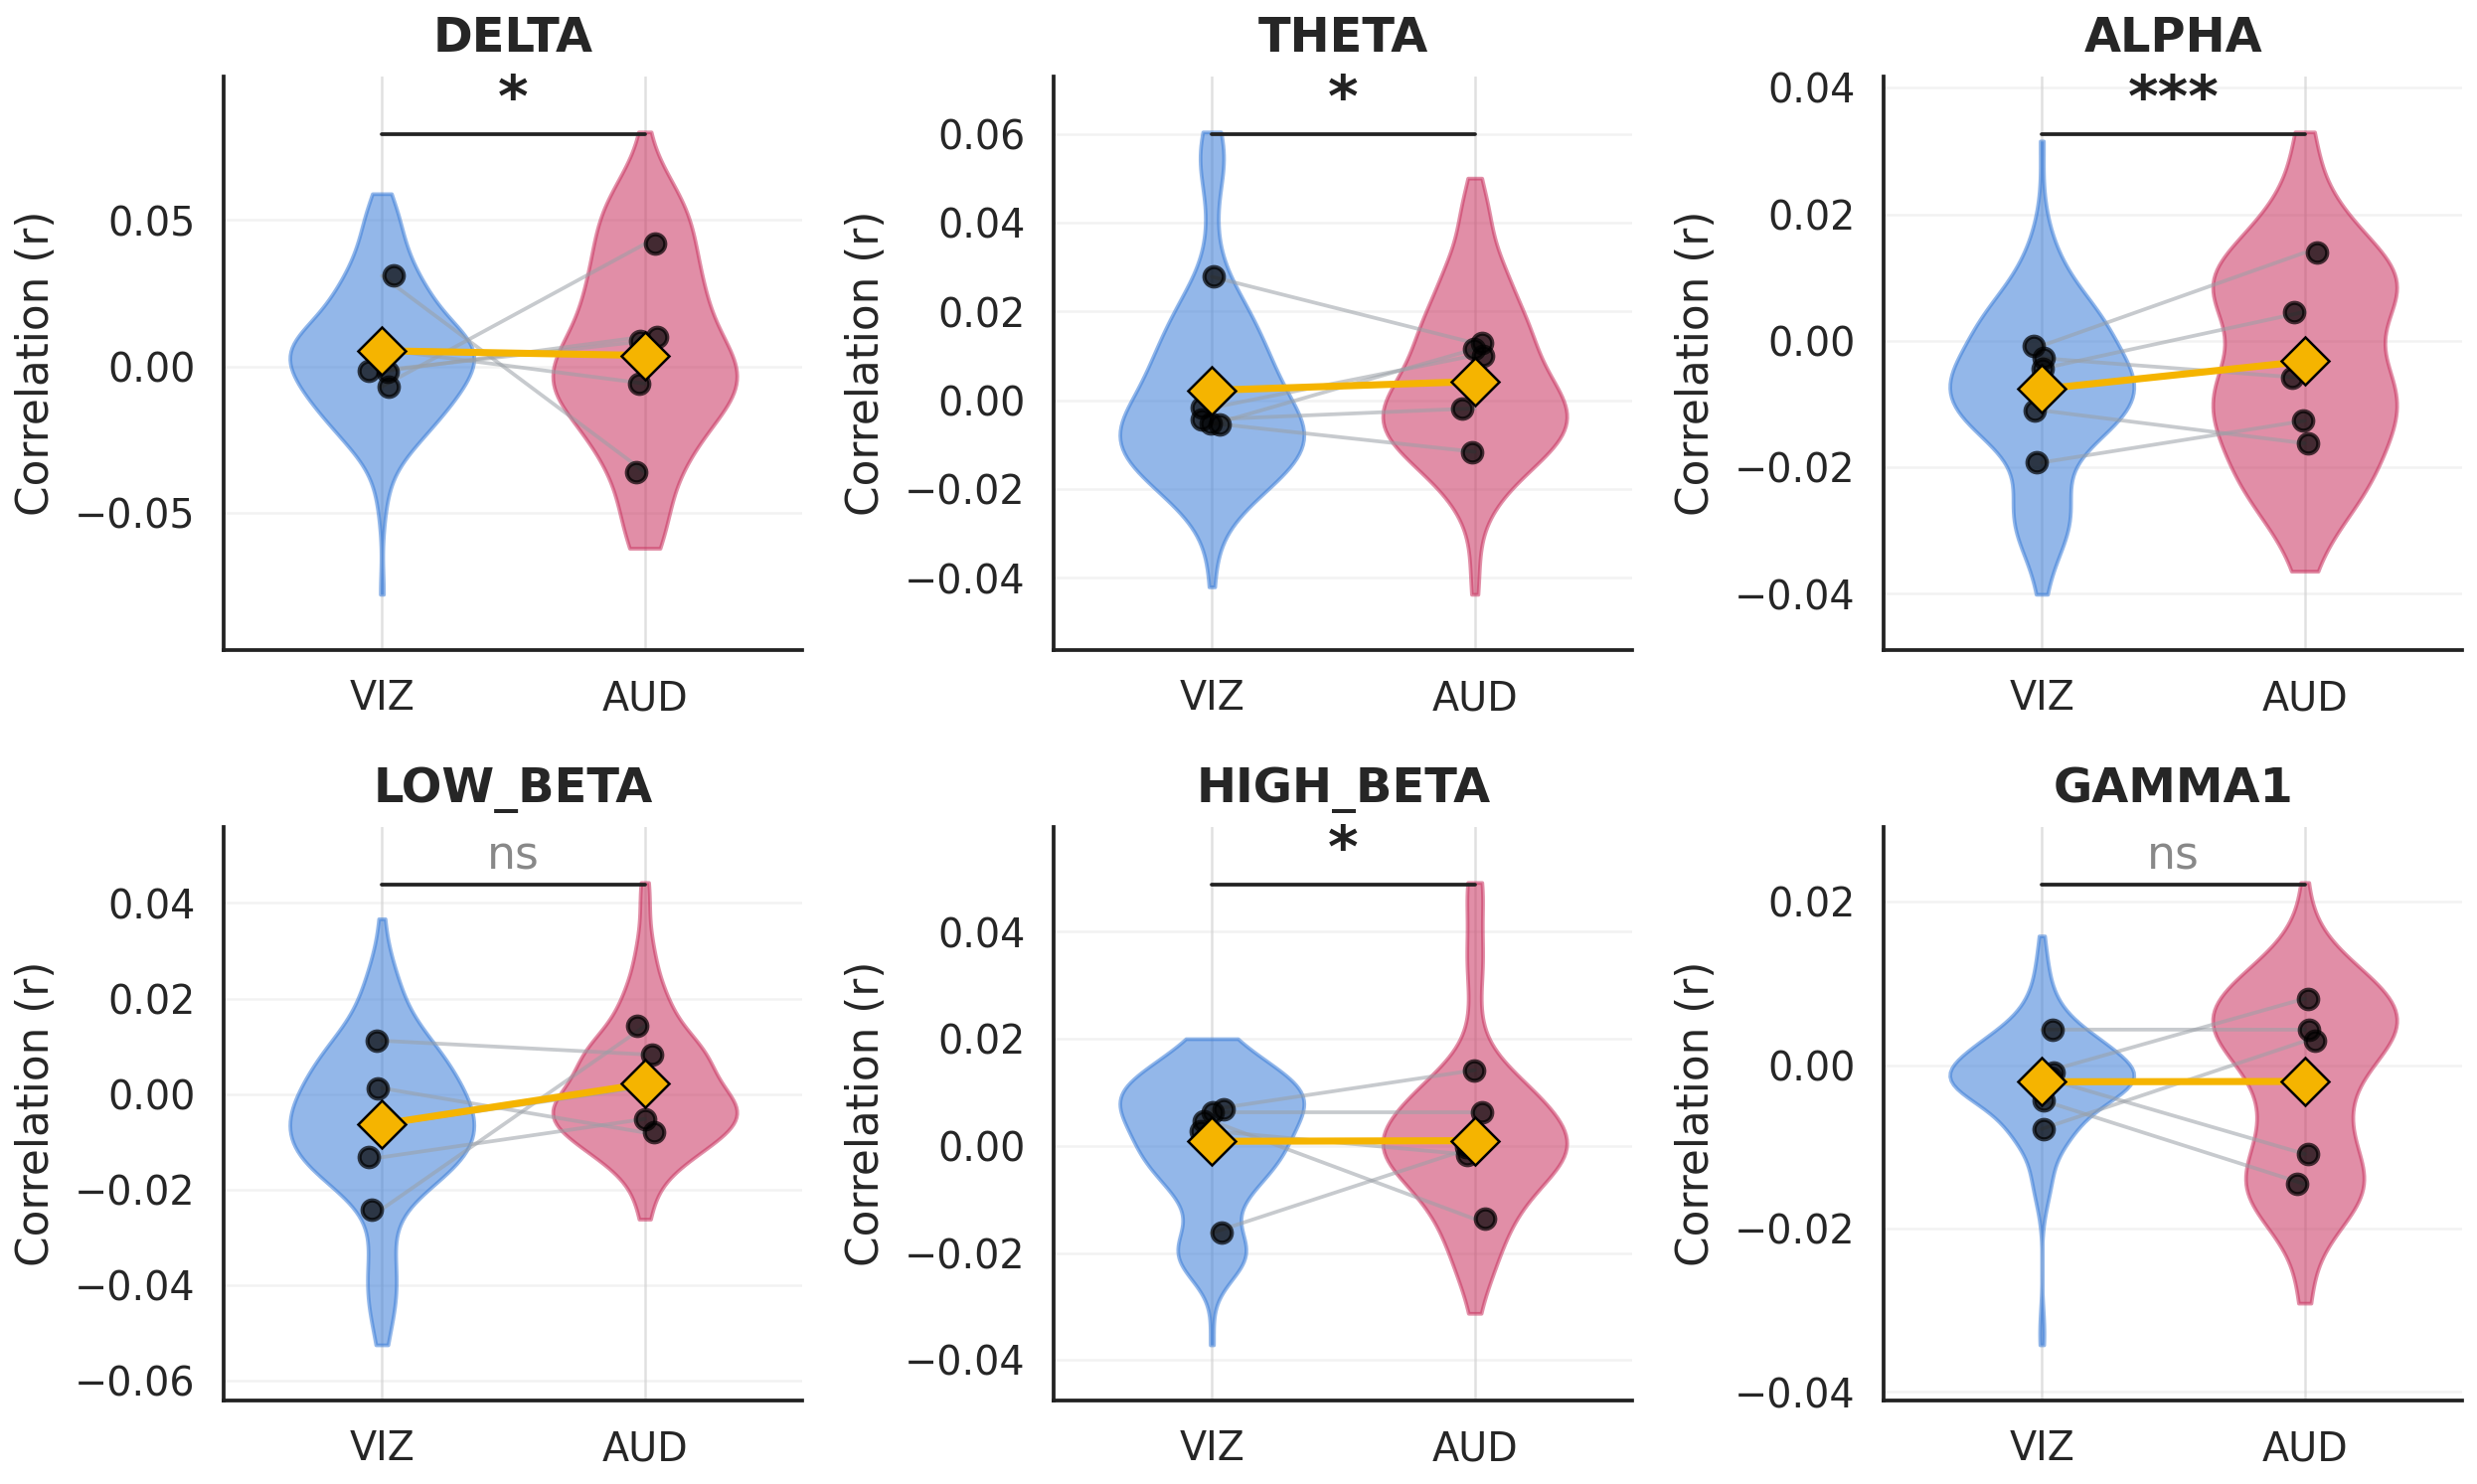
\includegraphics[width=0.96\linewidth]{Fig4_violins_VIZ_vs_AUD.png}
\caption{\textbf{EEG--audio envelope correlation: \textsc{viz} vs.\
\textsc{aud}, n=5 subjects $\times$ 32 channels.} Six EEG bands (delta
0.5--4, theta 4--8, alpha 8--13, low-beta 13--20, high-beta 20--30,
gamma$_1$ 30--50\,Hz). For each (subject, channel, band, condition) we
band-pass-filter both the audio amplitude envelope and the EEG to the
same band, then compute Pearson $r$ on the matched-rate signals. Each
panel shows the distribution of those per-(subject, channel) $r$ values
for \textsc{viz} (blue) and \textsc{aud} (rose); grey lines connect
within-channel paired values; gold diamond + line shows the channel-mean
trajectory. \emph{Statistical inference}: per-channel paired test with
condition as fixed effect; the resulting per-channel $p$-values are
Benjamini--Hochberg FDR-corrected within each band. Bracket annotation
``$N/32$ ch FDR$<$.05'' reports the count of channels surviving FDR per
band; the bracket star reflects the smallest band-level FDR-corrected
$p$. \textsc{viz} vs.\ \textsc{aud} shows broadband effects: 30/32 ch
delta ($*$), 5/32 theta ($*$), 32/32 alpha (\texttt{***}), 11/32
high-beta ($*$); low-beta and gamma$_1$ ns.}
\label{fig:Fig4_VA}
\end{figure}

\begin{figure}[H]
\centering
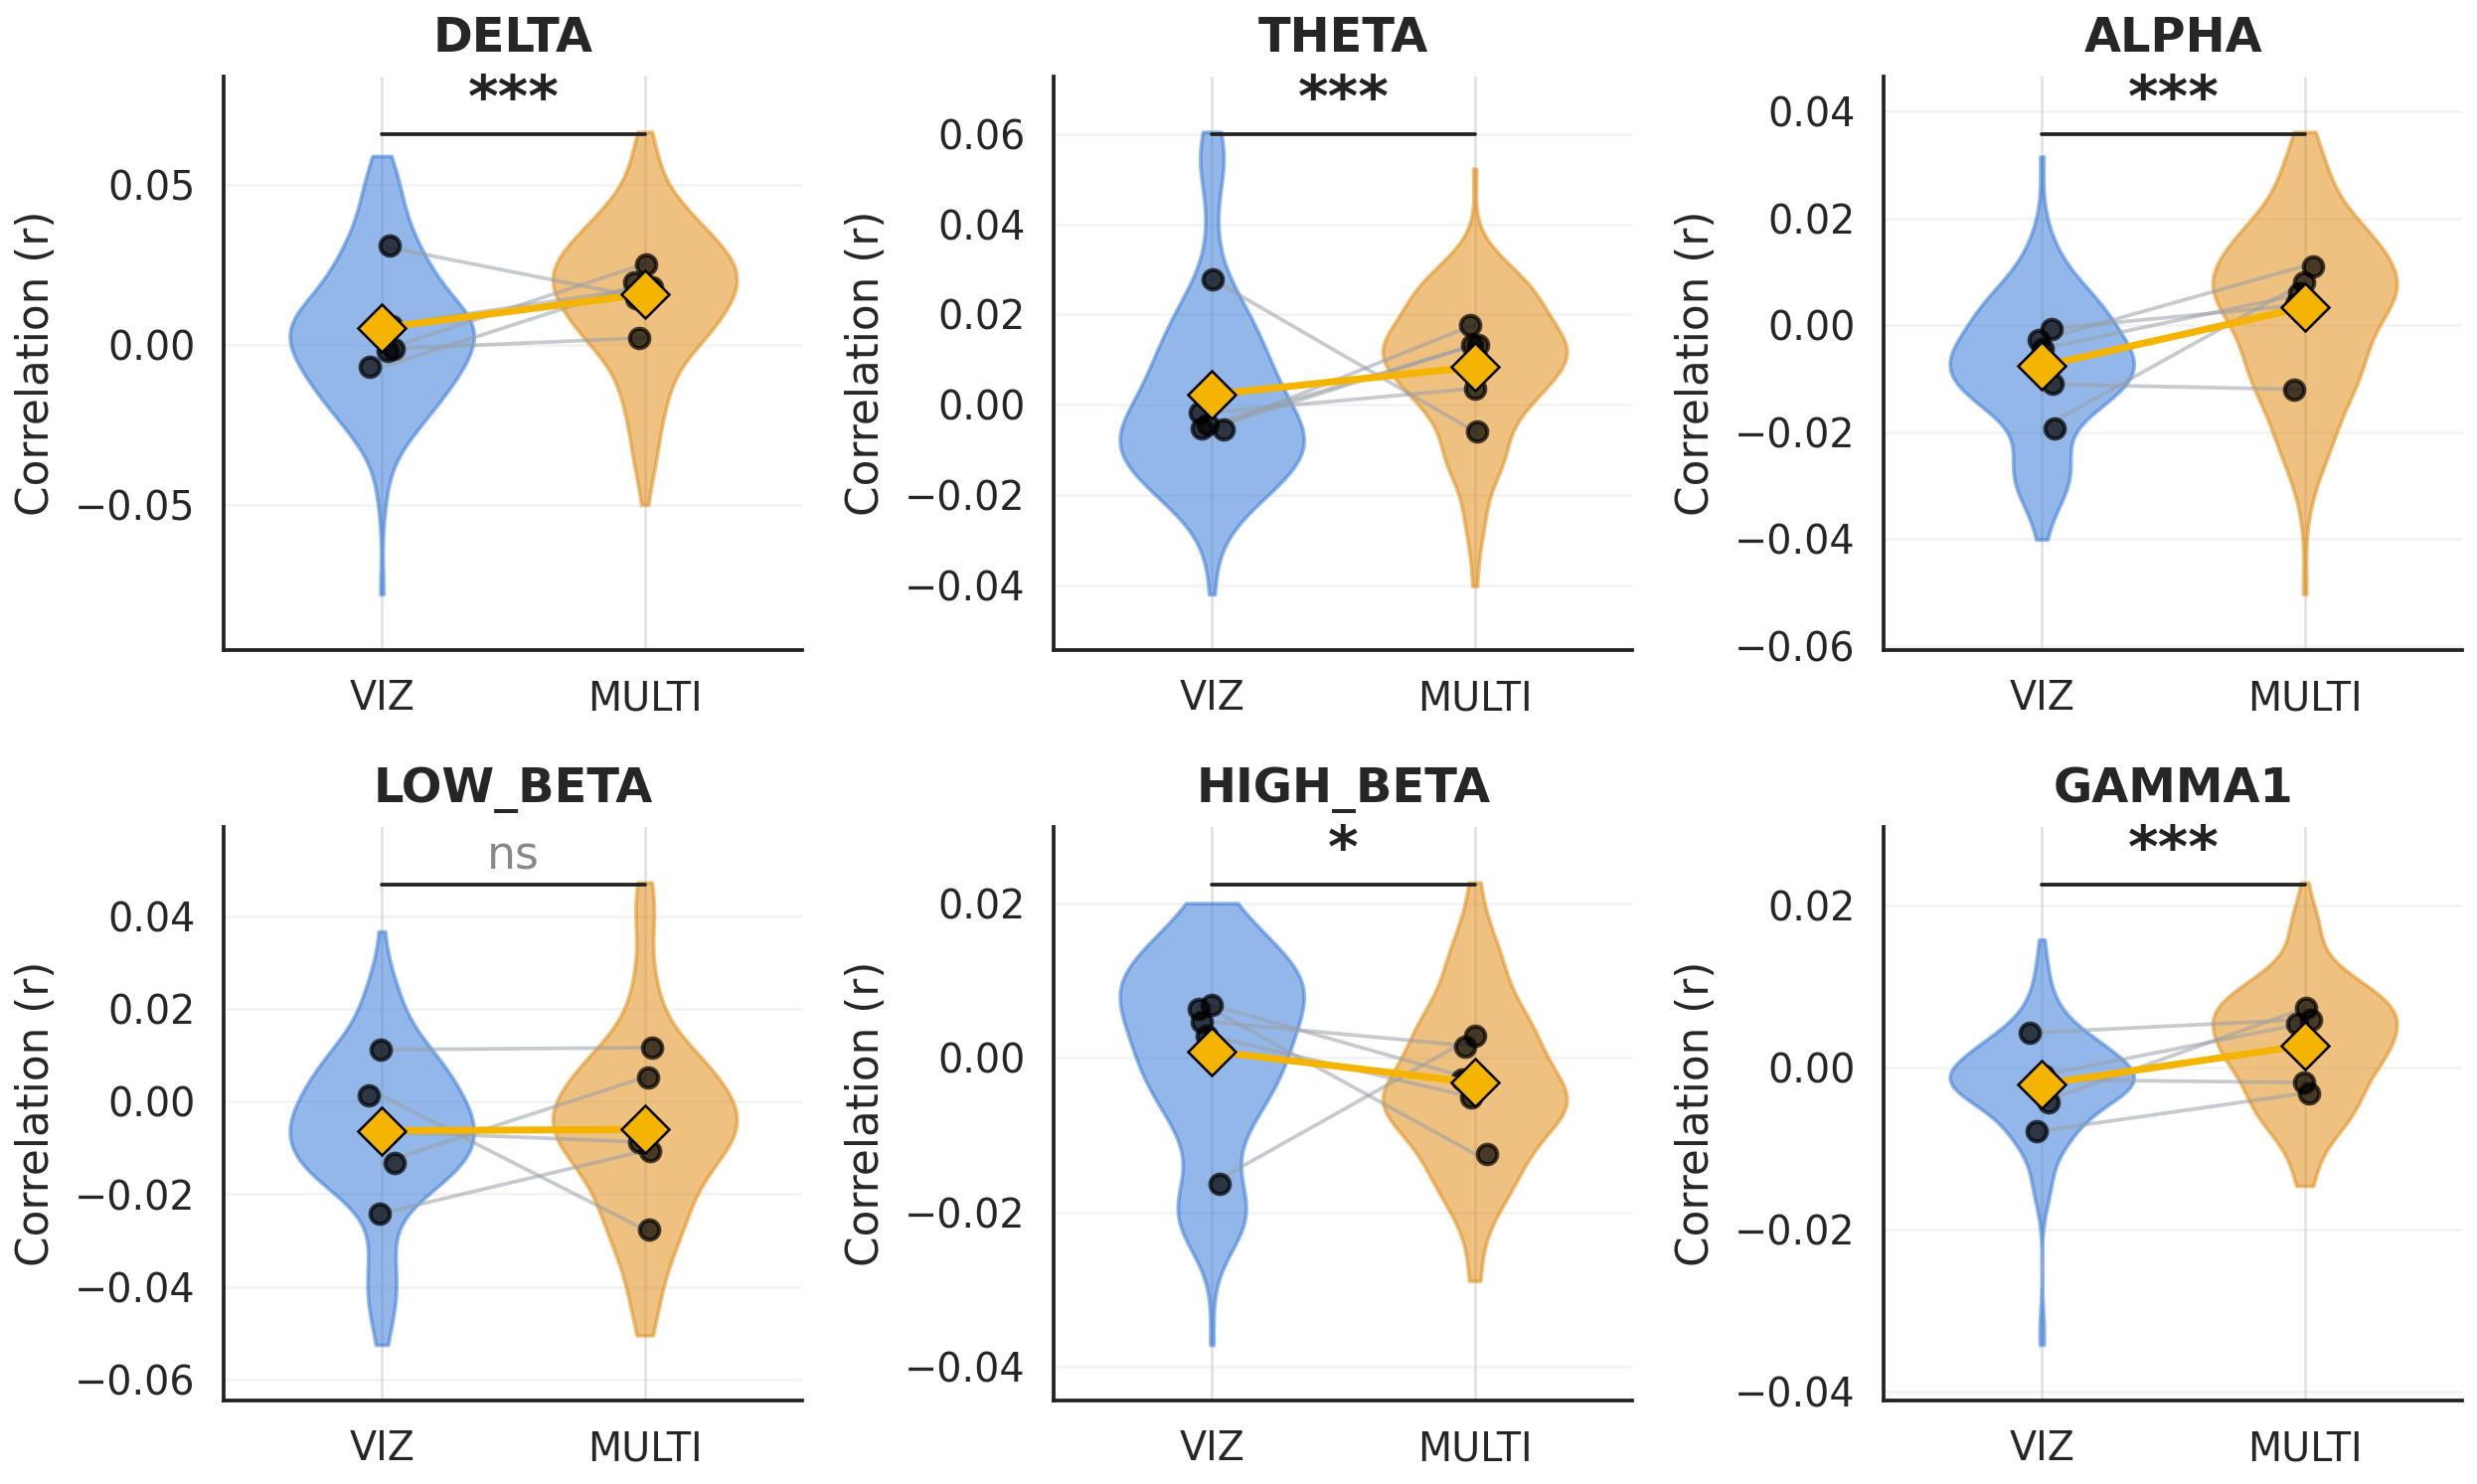
\includegraphics[width=0.96\linewidth]{Fig4_violins_VIZ_vs_MULTI.png}
\caption{\textbf{EEG--audio envelope correlation: \textsc{viz} vs.\
\textsc{multi}, n=5 subjects $\times$ 32 channels.} Same layout, filters
and statistical apparatus (per-channel paired test + BH-FDR within band)
as Figure~\ref{fig:Fig4_VA}. Notable counts: 7/32 ch delta ($*$), 23/32
theta (\texttt{**}), 0/32 alpha (ns), 0/32 low-beta (ns), 0/32 high-beta
(ns), 24/32 gamma$_1$ (\texttt{**}).}
\label{fig:Fig4_VM}
\end{figure}

\begin{figure}[H]
\centering
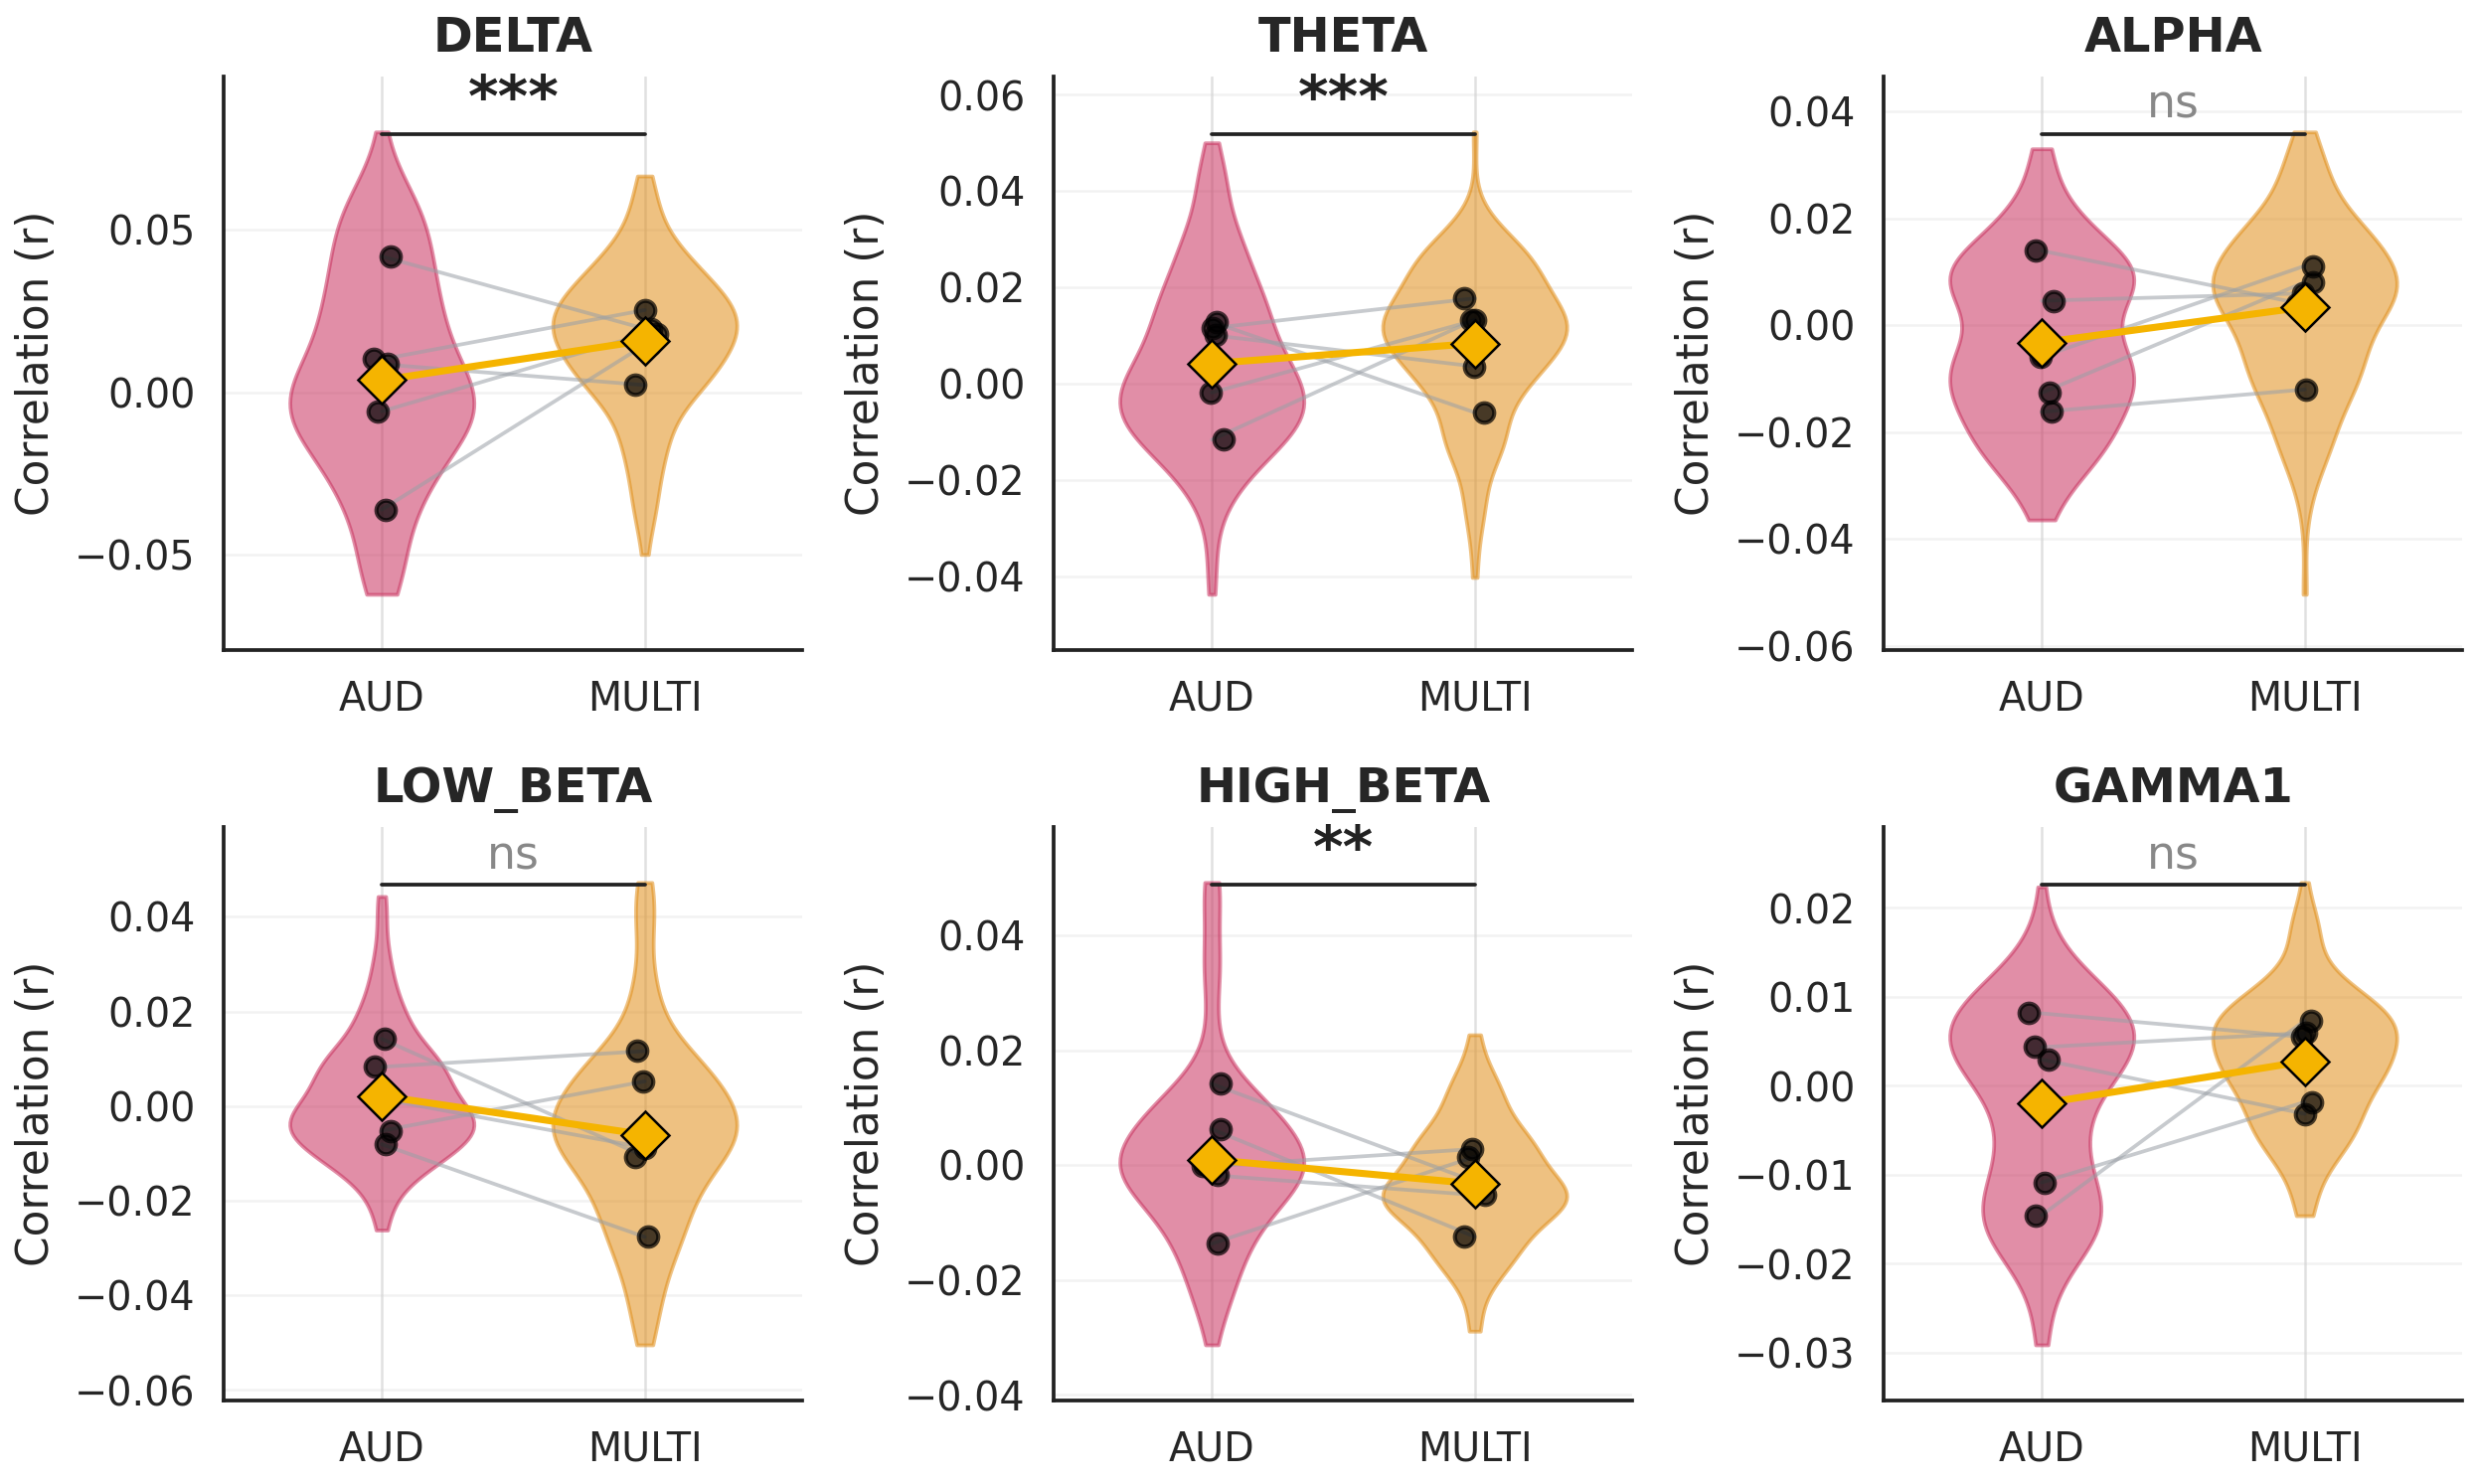
\includegraphics[width=0.96\linewidth]{Fig4_violins_AUD_vs_MULTI.png}
\caption{\textbf{EEG--audio envelope correlation: \textsc{aud} vs.\
\textsc{multi}, n=5 subjects $\times$ 32 channels.} Same layout, filters
and statistical apparatus (per-channel paired test + BH-FDR within band)
as Figure~\ref{fig:Fig4_VA}. Notable counts: 1/32 ch delta (ns),
32/32 theta (\texttt{***}), 0/32 alpha (ns), 0/32 low-beta (ns),
26/32 high-beta (\texttt{***}), 0/32 gamma$_1$ (ns).}
\label{fig:Fig4_AM}
\end{figure}

\section{Discussion}

Three results stand out at the pilot stage. \emph{(i)} Respiration is the
fastest physiological channel to lock to slow audio rhythms: PLV and wPLI
between respiration and the audio swell are higher during nature listening
than during silence (LMM-windowed $p\!<\!0.05$), and the locking peaks under
audio-only stimulation, where attention is undivided. \emph{(ii)} Slow
cardiac rhythms (mean RR interval) decouple from the very-slow swell
(0.1\,Hz) when nature audio is presented, suggesting that the heart's
intrinsic VLF/LF drift loses its incidental alignment with sub-respiratory
audio carriers as soon as the body engages with the sound. \emph{(iii)}
Linear methods (cross-correlation, coherence) under-detect what phase
methods (PLV, wPLI) and information-theoretic methods (MI on Hilbert
envelopes) recover, especially on the slow envelope columns --- a useful
prior for analysis choices in the larger study.

The phase-clustering analysis is the cleanest small-sample test we have:
under audio-only listening, 4/5 subjects show within-subject phase
consistency \emph{and} the group converges on a common phase (Rayleigh
$R=0.73$). Under audio-visual co-stimulation, individual subjects still
lock internally but their phases scatter across the group --- consistent
with a picture in which visual stimulation pulls each subject's preferred
respiratory phase in idiosyncratic directions.

EEG--audio band-matched amplitude coupling shows broad band-specific
differences between conditions, but these are computed on the same data and
their interpretation depends on the sensory contrast: e.g.\
\textsc{multi}$>$\textsc{aud} on theta and high-beta is consistent with
multisensory binding overhead, not with simple stimulus tracking.

The largest methodological lessons for the planned full study are: (1)
phase metrics on the slow swell envelope should be the primary
respiration--audio readout; (2) HRV coupling should be reported separately
on the LF and HF envelopes (the swell-versus-nature direction differs); (3)
EEG analyses should plan for both the pseudoreplication-aware LMM (subject
$\times$ channel crossed random effects) and a small-N-honest paired test on
subject means.

\paragraph{Limitations.} n=5, two recording sites (Chile, Mallorca), single session
per subject, no behavioural / phenomenological measures yet, no fractal
analyses yet --- all of which are addressed in the planned design. The pilot
narrowly establishes the methodological feasibility of the multimodal
coupling pipeline rather than testing the project's hypotheses at full
strength.

\bibliographystyle{plainnat}
\renewcommand{\refname}{References}

\begin{thebibliography}{99}

\bibitem[Bratman et al.(2015)]{bratman2015}
Bratman, G.\,N., Daily, G.\,C., Levy, B.\,J., \& Gross, J.\,J. (2015).
The benefits of nature experience: Improved affect and cognition.
\textit{Landscape and Urban Planning}, 138, 41--50.

\bibitem[Carpentier(2020)]{carpentier2020}
Carpentier, S. (2020). Complexity matching: Brain signals mirror environment
information patterns during music listening and reward. \textit{Journal of
Cognitive Neuroscience}, 32(4), 734--745.

\bibitem[Gordon et al.(2017)]{gordon2017}
Gordon, N., Koenig-Robert, R., Tsuchiya, N., Van Boxtel, J.\,J.,
\& Hohwy, J. (2017). Neural markers of predictive coding under perceptual
uncertainty revealed with hierarchical frequency tagging. \textit{eLife},
6, e22749.

\bibitem[Hartig et al.(2014)]{hartig2014}
Hartig, T., Mitchell, R., de Vries, S., \& Frumkin, H. (2014). Nature and
health. \textit{Annual Review of Public Health}, 35, 207--228.

\bibitem[Lakatos et al.(2008)]{lakatos2008}
Lakatos, P., Karmos, G., Mehta, A.\,D., Ulbert, I., \& Schroeder, C.\,E.
(2008). Entrainment of neuronal oscillations as a mechanism of attentional
selection. \textit{Science}, 320(5872), 110--113.

\bibitem[Mayer \& Frantz(2004)]{mayer2004}
Mayer, F.\,S., \& Frantz, C.\,M. (2004). The connectedness to nature scale:
A measure of individuals' feeling in community with nature. \textit{Journal
of Environmental Psychology}, 24(4), 503--515.

\bibitem[Nozaradan et al.(2011)]{nozaradan2011}
Nozaradan, S., Peretz, I., Missal, M., \& Mouraux, A. (2011). Tagging the
neuronal entrainment to beat and meter. \textit{Journal of Neuroscience},
31(28), 10234--10240.

\bibitem[Taylor \& Spehar(2016)]{taylor2016}
Taylor, R.\,P., \& Spehar, B. (2016). Fractal fluency: An intimate
relationship between the brain and processing of fractal stimuli.
In \textit{The Fractal Geometry of the Brain} (pp.\ 485--496). Springer.

\end{thebibliography}

\end{document}
